%!TEX root = ../main.tex
\chapter{Cross-check of the calibration}
\label{chap:TimingValidation}

The timing calibration procedure was presented in chapter \ref{chap:TimingCalib}. In order to validate the calibration, the recorded electron data is used. Electromagnetic showers are quasi-instantaneous and perfect to cross-check the time calibration procedure. The selection applied to the electron data sample is described in section \ref{subsec:elec_sel}. The same calibration constants and correction constants determined from the muon data are applied to the electron data.

\section{Time of the first hit for electrons}

The time of the first hit for 20 GeV electrons is shown in figure \ref{fig:Timing_electrons}. The time distribution presents a large tail to the right and is much wider than for muons. This indicates that an effect is present in electron data but not in muon data. The difference seen could be related to the fact that in electromagnetic showers, the number of hits is much higher than for muons as well as the energy deposited in a single cell can be over hundreds MIP.

Additionally, a timing offset of around 10 ns can be seen. This is expected and it is consistent with the changes in trigger configuration from the big scintillator plates to the small trigger scintillator of $10\times10$ cm$^2$.

\begin{figure}[htbp!]
	\centering
	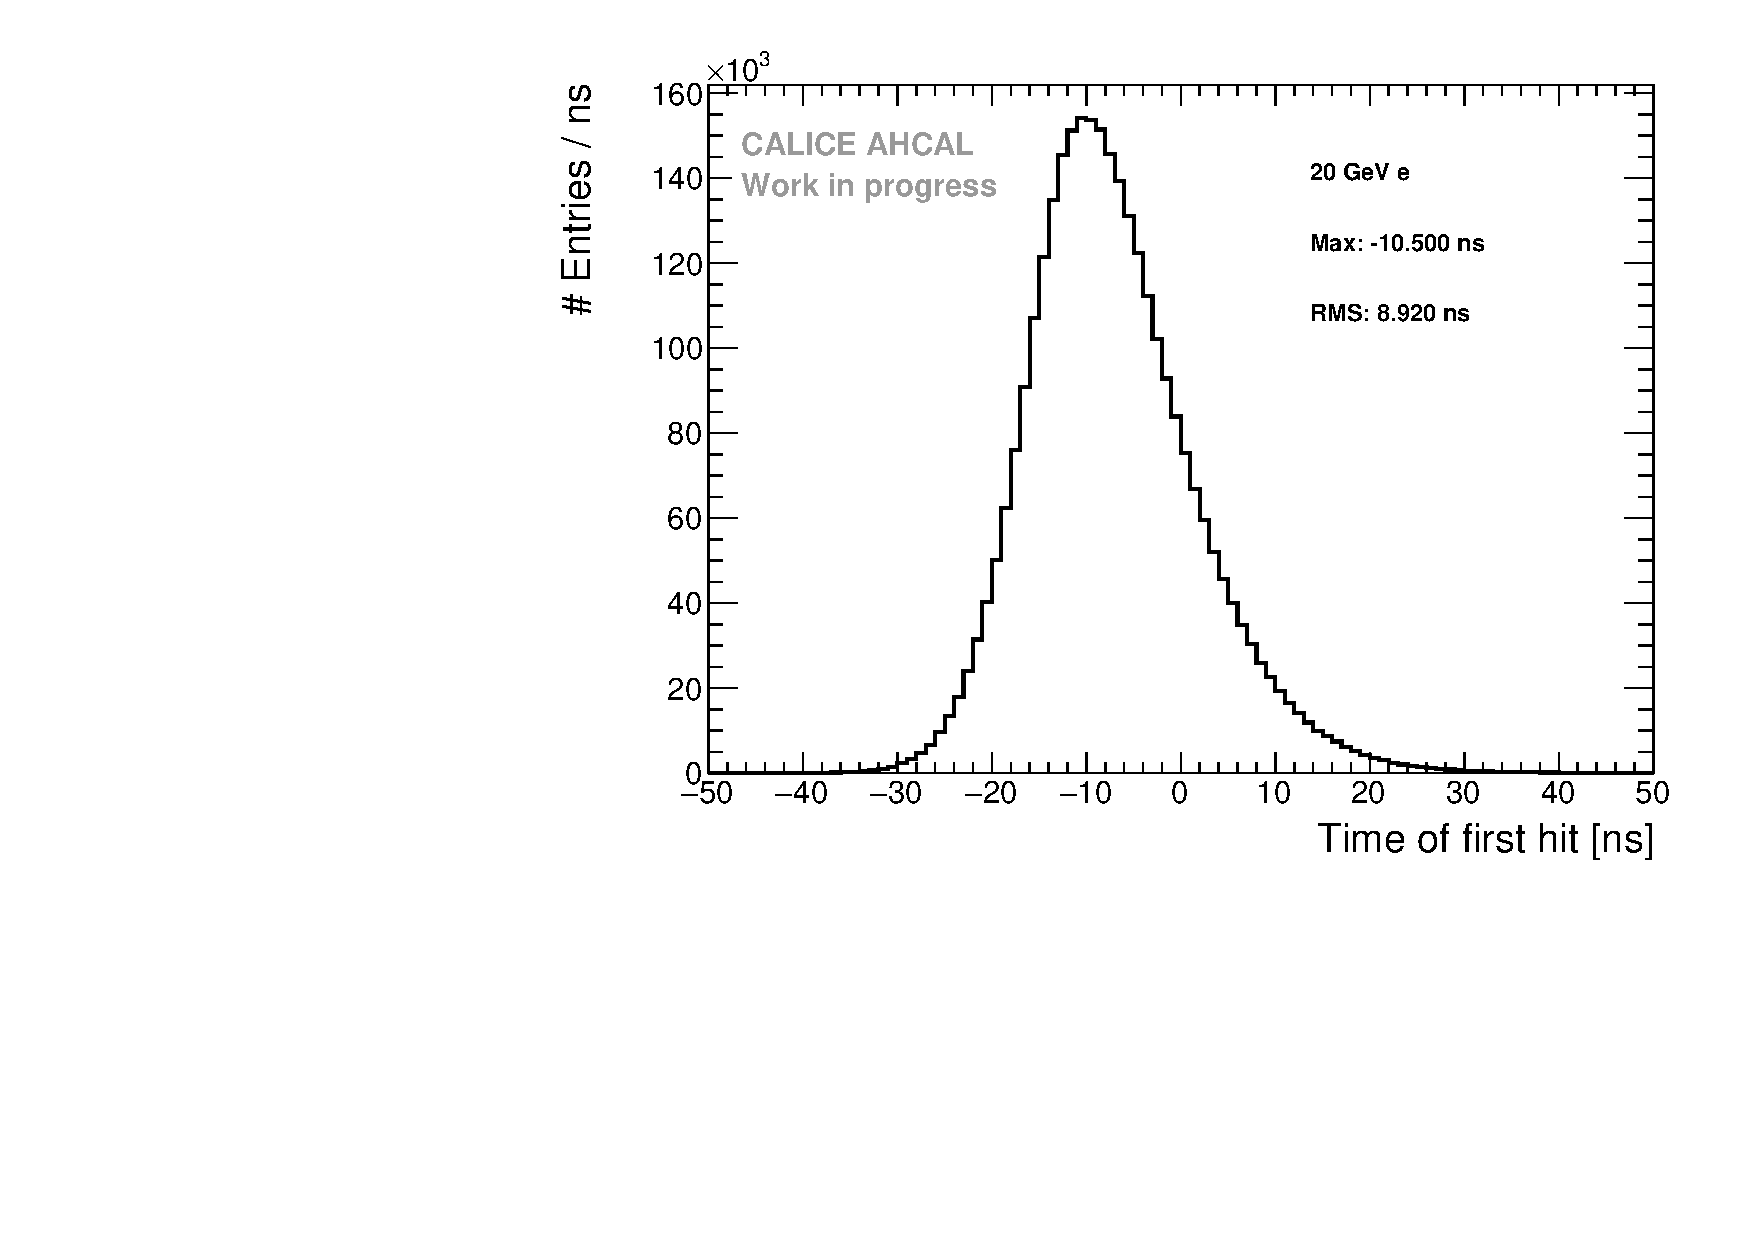
\includegraphics[width=0.5\textwidth]{../Thesis_Plots/Timing/Electrons/Plots/Timing_AllLayers_AfterMuons.pdf}
	\caption{Time of the first hit distribution for 20 GeV electrons after applying the calibration constants extracted from the muon data, before further corrections. Max = -10.05 ns, RMS = 8.92 ns.}
	\label{fig:Timing_electrons}
\end{figure}

\section{Influence of the number of triggered channels}
\label{subsec:ped_shift}

For the energy measurement, pedestal shift is a known feature of the \textit{SPIROC2B} chip \cite{Hartbrich2012}. This electronic effect that induces a shift in the baseline of the ADC signal may be also present for the timing measurement. It has been investigated by looking at the time of the first hit as a function of the number of triggered channels over 0.5 MIP. The correction should not be beam energy dependent and all electron beam energies are used to determine the correction.

The time of first hit as a function of the number of triggered channels over 0.5 MIP is shown in figure \ref{fig:nhits_profile}. The effect on the measured hit time can be very large, a correction up to 30-40 ns can be necessary to the data for a high number (15-20) of triggered channels above 0.5 MIP. The cause of the observed effect is most likely due to an element in the chip called a \textit{delay box} that gets unstable with a high number of triggered channels. This chip element is responsible for the hold signal of the TDC ramp in the chip. The hold signal is delayed, and thus a higher TDC ramp value than the one expected is sampled.

\begin{figure}[htbp!]
	\begin{subfigure}[t]{0.5\textwidth}
		\centering
		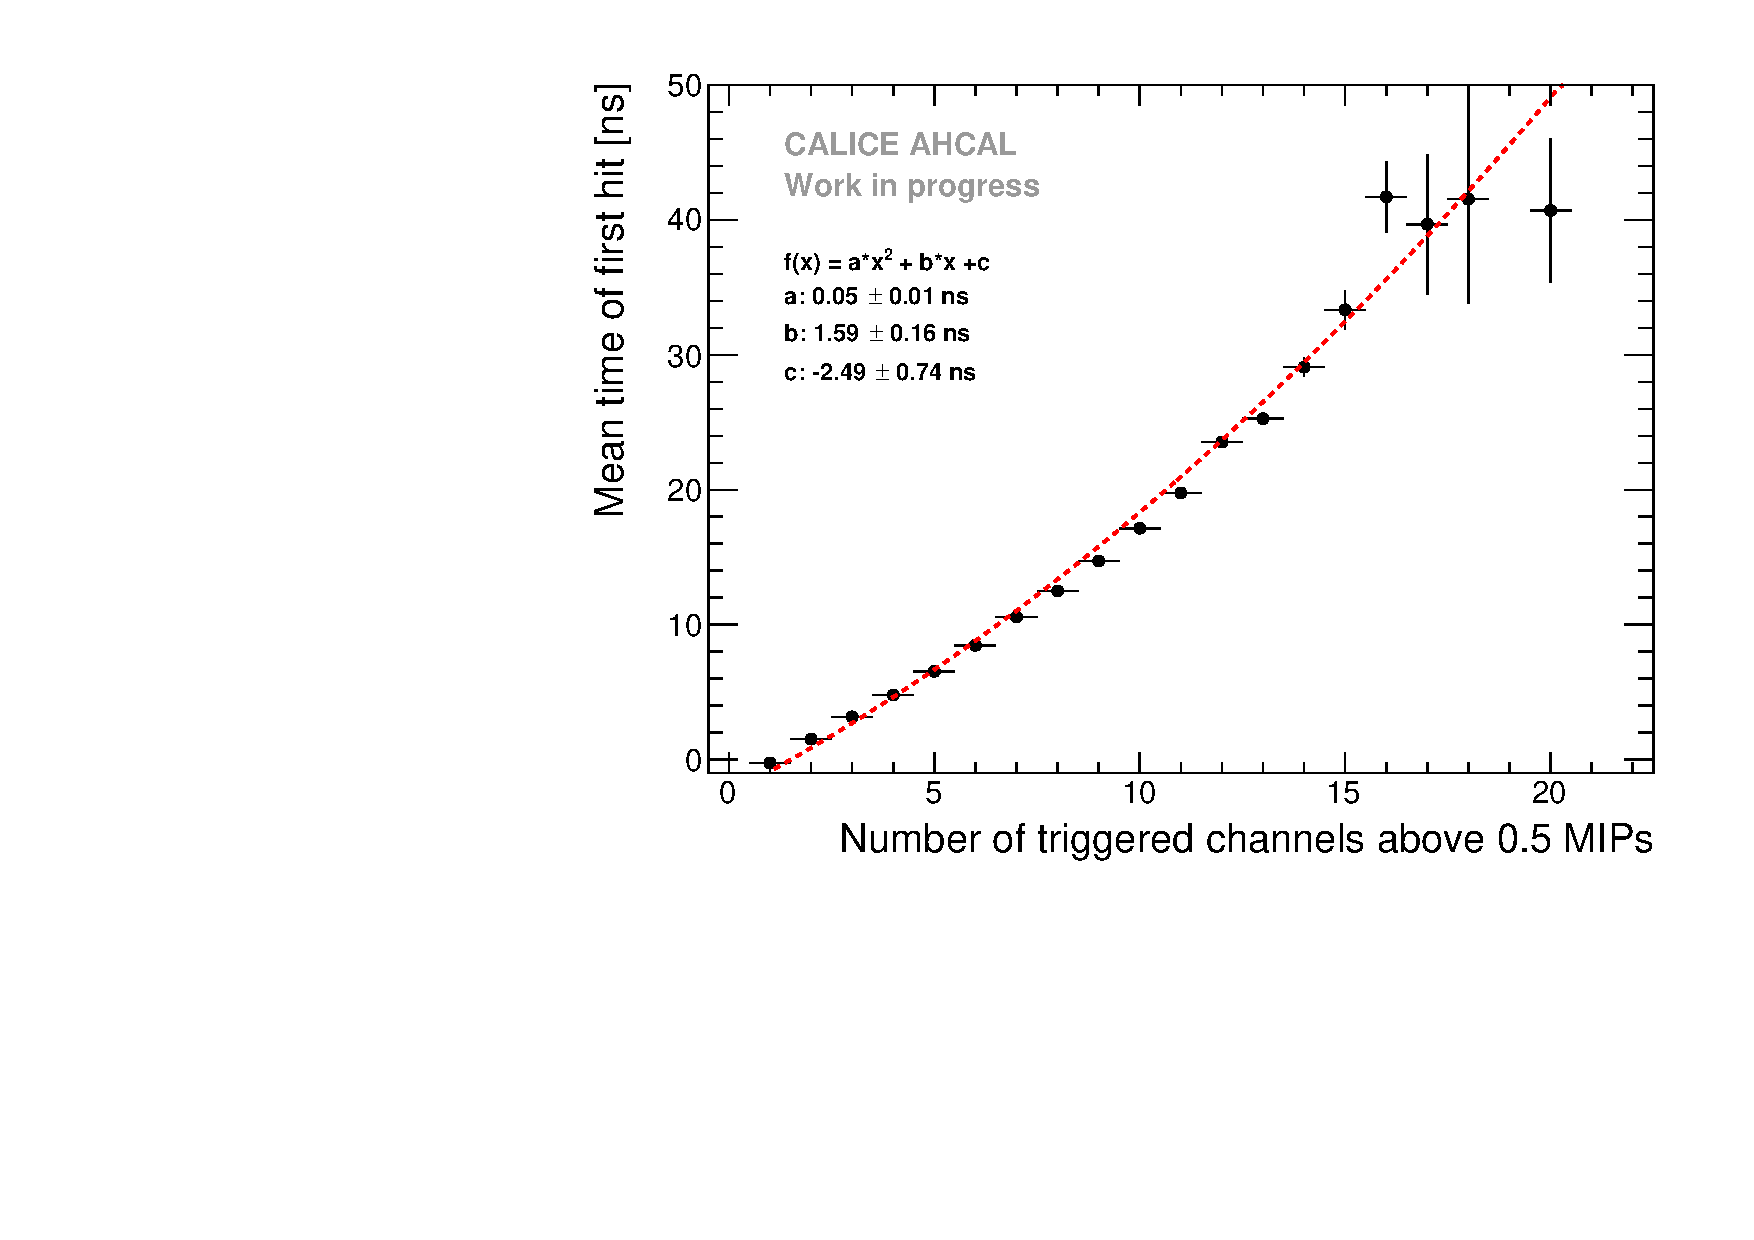
\includegraphics[width=1\textwidth]{../Thesis_Plots/Timing/Electrons/Plots/NumberHits_Dependance_AllEnergies.pdf}
		\caption{}\label{fig:nhits_profile}
	\end{subfigure}
	\hfill
	\begin{subfigure}[t]{0.5\textwidth}
		\centering
		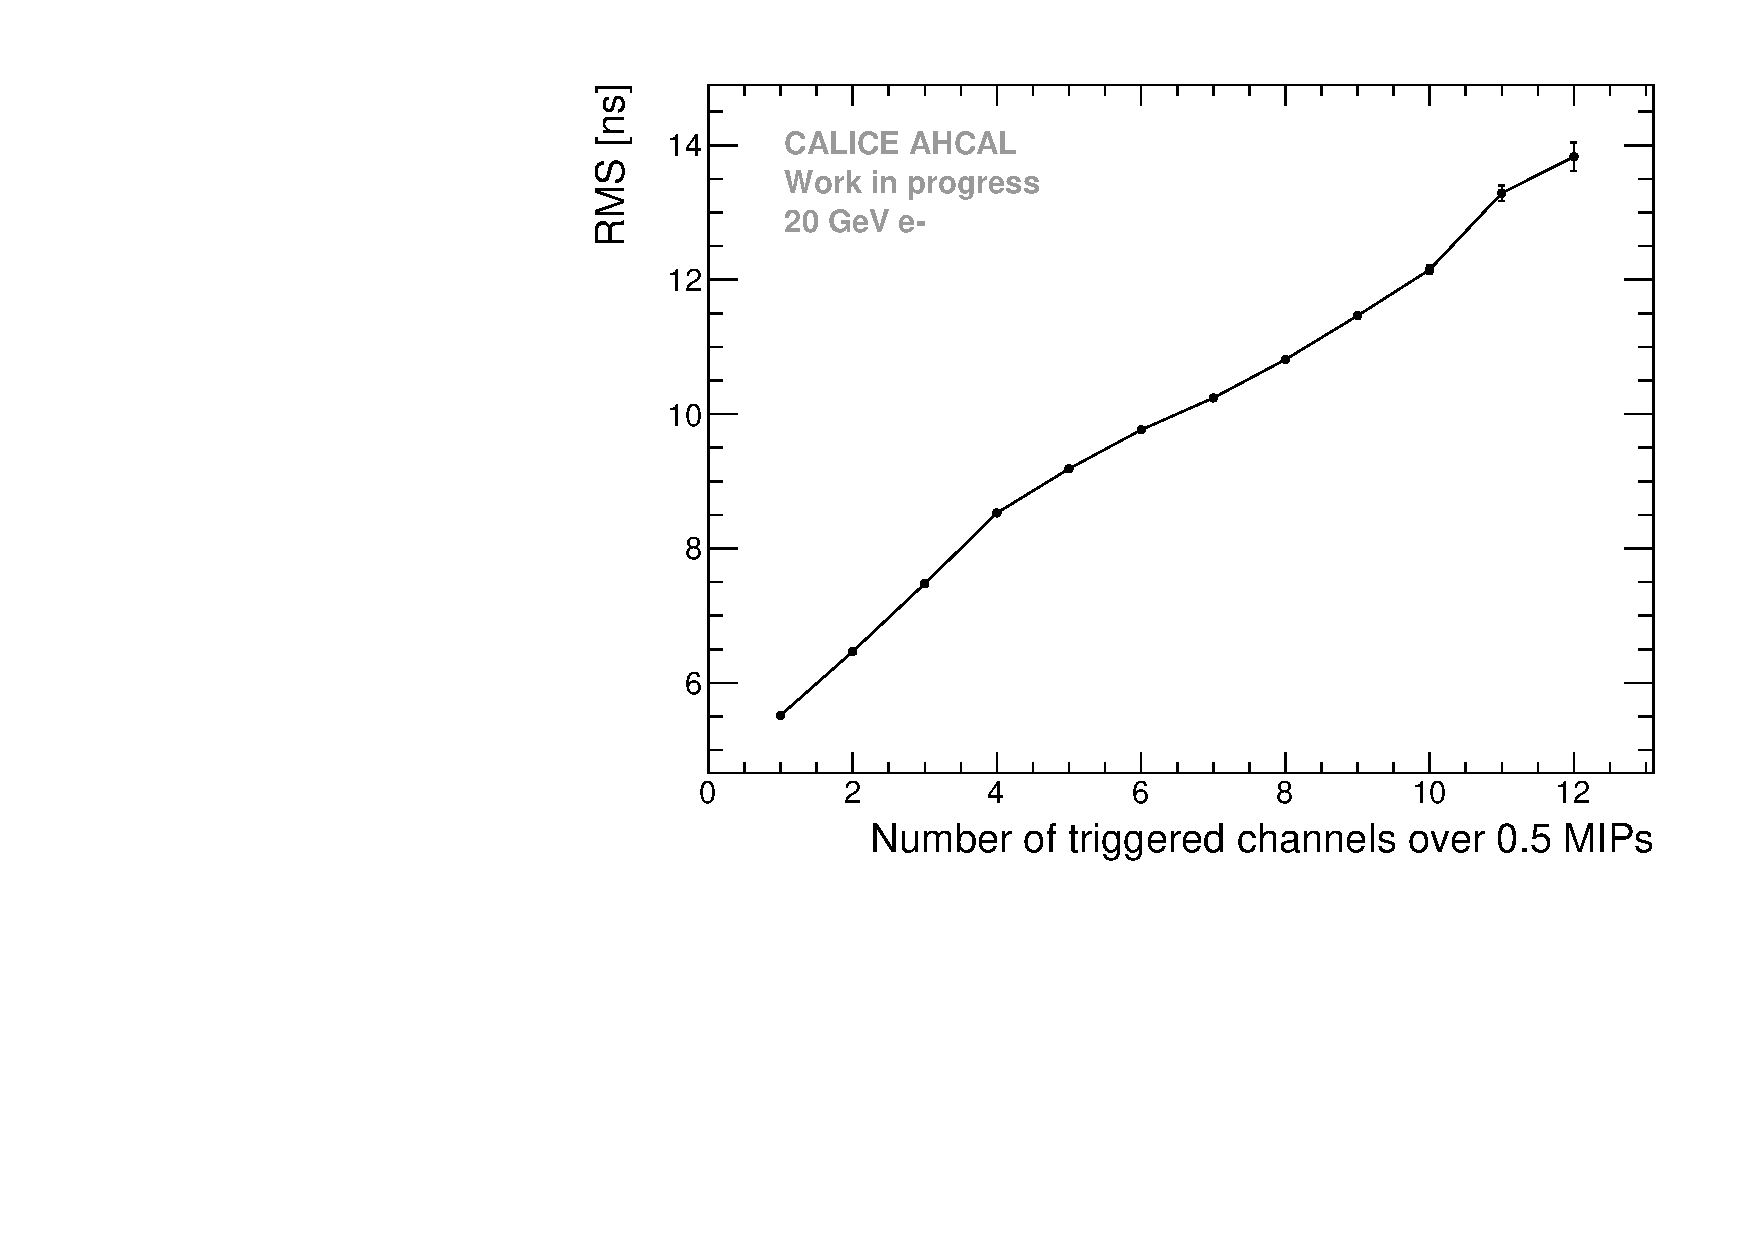
\includegraphics[width=1\textwidth]{../Thesis_Plots/Timing/Electrons/Plots/ParametrisationPedestalShift_20GeV.pdf}
		\caption{}\label{fig:RMS_nHits}
	\end{subfigure}
	\caption{\subref{fig:nhits_profile}) Mean time of the first hit as a function of the number of triggered channels above 0.5 MIP in a chip. The mean time shift upwards with the increase of triggers leading to large tails in the time distribution. The plot is obtained by combining all electron energies and a second order polynomial fit is done. \subref{fig:RMS_nHits}) The RMS of the time of first hit as a function of the number of triggered channels above 0.5 MIP for 20 GeV electrons. The RMS of the time distribution can increase up to 10-15 ns for a high number of triggered channels.}
\end{figure}

The correction parameters are determined by a polynomial fit to the data. In addition, this effect does not only shift the mean of the time distribution but also increases its width. The width increases with the number of triggered channels in a chip, therefore making the time resolution of the AHCAL dependent on the number of hits. This is shown in figure \ref{fig:RMS_nHits}.

As expected, if only a single channel triggers in a chip, the time resolution is close to the timing resolution obtained for muons. Additionally, since it is a priori not clear if the effect depends on the number of triggered channels in a chip or the energy sum in a chip, the correction has been checked using both variables. But the correction is better as a function of the number of triggered channels in a chip.

\section{Time of the first hit for electrons}
\label{subsec:Electron_Final}

After applying the correction as function of the number of triggered channels in a chip, the distribution of the time of the first for 20 GeV electrons has been investigated as shown in figure \ref{fig:timing_electrons_corr}. The correction improves the RMS of the distribution by around 12.1\%, as well as the distribution appears more Gaussian-like.

However, there is still a discrepancy of around 33.7\% with the time resolution obtained with muons of around 5.36 ns (see section \ref{subsec:Muon_final}). This is because of the increase of the RMS of the time distribution as a function of the number of triggered channels in a chip as seen in figure \ref{fig:RMS_nHits}. The increase of the RMS can't be corrected unlike the mean of the time distribution.

In order for the simulation to match the data, the increase of the width of the time distribution has to be parametrized from the data. More details about the parametrization implementation in the simulation are in the appendix \ref{appendix:ped_shift}.

\begin{figure}[htbp!]
	\begin{subfigure}[t]{0.5\textwidth}
		\centering
		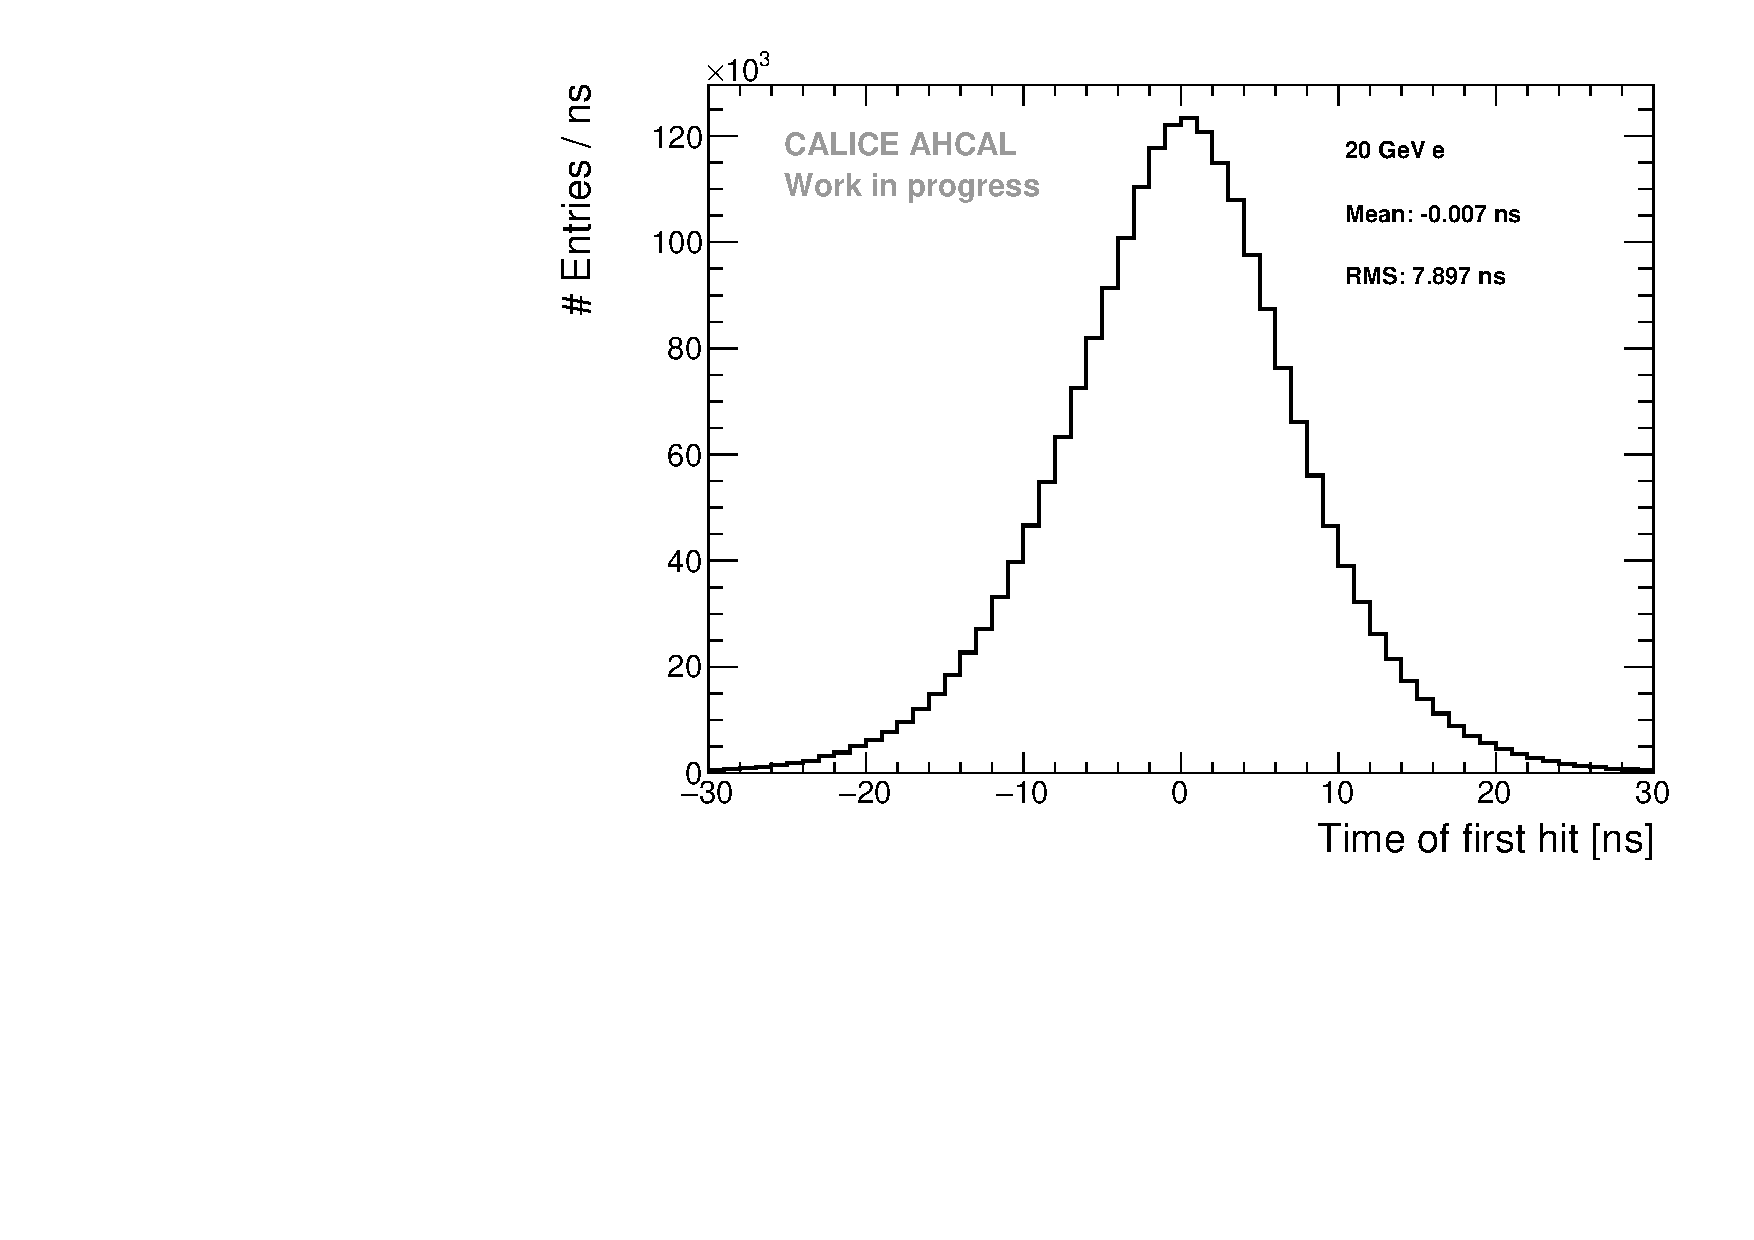
\includegraphics[width=1\textwidth]{../Thesis_Plots/Timing/Electrons/Plots/Timing_AllLayers_20GeV.pdf}
		\caption{}\label{fig:timing_electrons_corr}
	\end{subfigure}
	\hfill
	\begin{subfigure}[t]{0.5\textwidth}
		\centering
		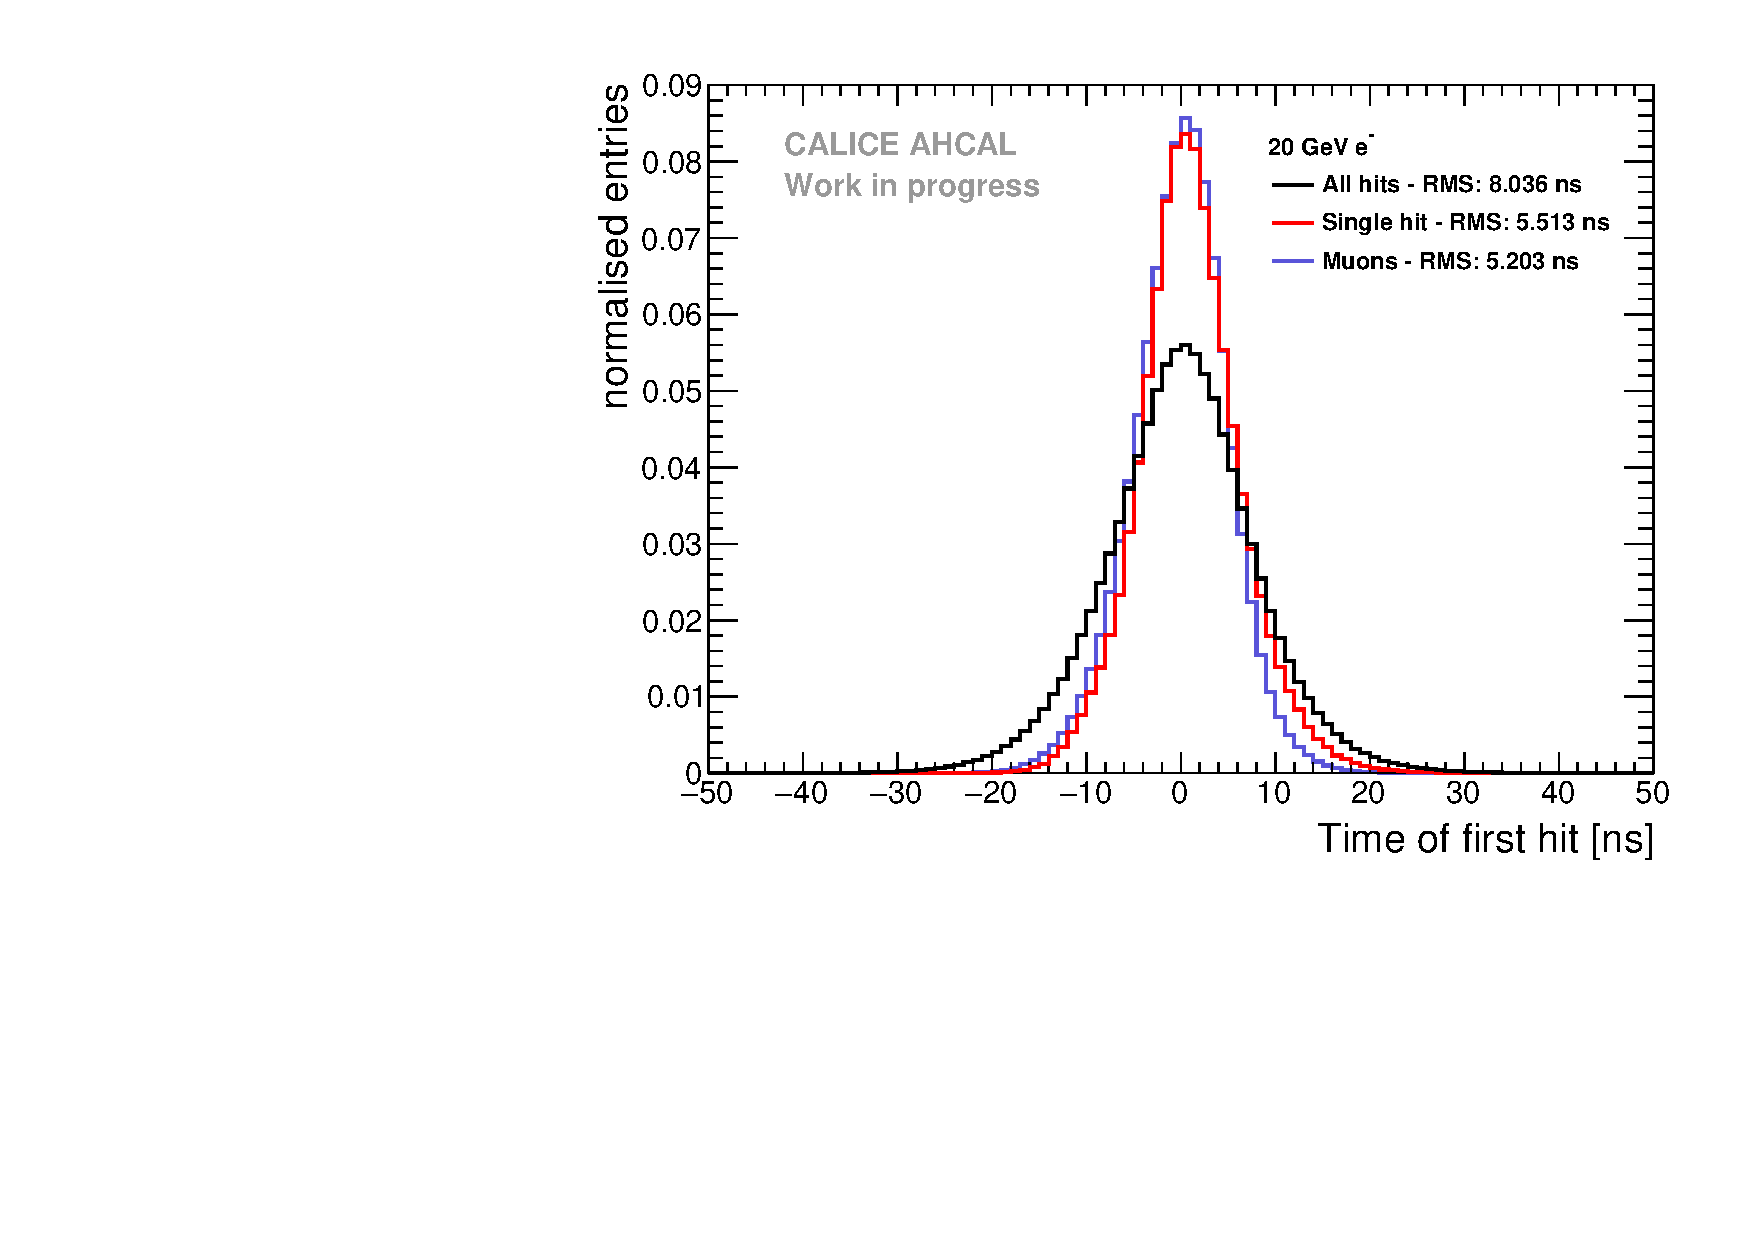
\includegraphics[width=1\textwidth]{../Thesis_Plots/Timing/Electrons/Plots/ComparisonAll_ElectronsSingleHit.pdf}
		\caption{}\label{fig:timing_electron_muon_comp}
	\end{subfigure}
	\caption{\subref{fig:timing_electrons_corr}) Time of the first hit distribution for 20 GeV electrons after the number of triggered channel correction, $\mu$ = -0.018 ns, RMS = 7.84 ns. \subref{fig:timing_electron_muon_comp}) Comparison of the 20 GeV electron sample with the muon time distribution for the time of first hit distribution. The time distribution is very similar to the distribution obtained with muons if only events in which only single hits in a chip are taken.}
\end{figure}

A comparison with the muon data has been done in order to further cross-check the calibration as well as the correction. The comparison is shown in figure \ref{fig:timing_electron_muon_comp}. If only event in which single hits in a chip are taken, the time resolution obtained is very similar to the time resolution observed with muons. The difference is around 5.2\%.

\begin{figure}[htbp!]
	\centering
	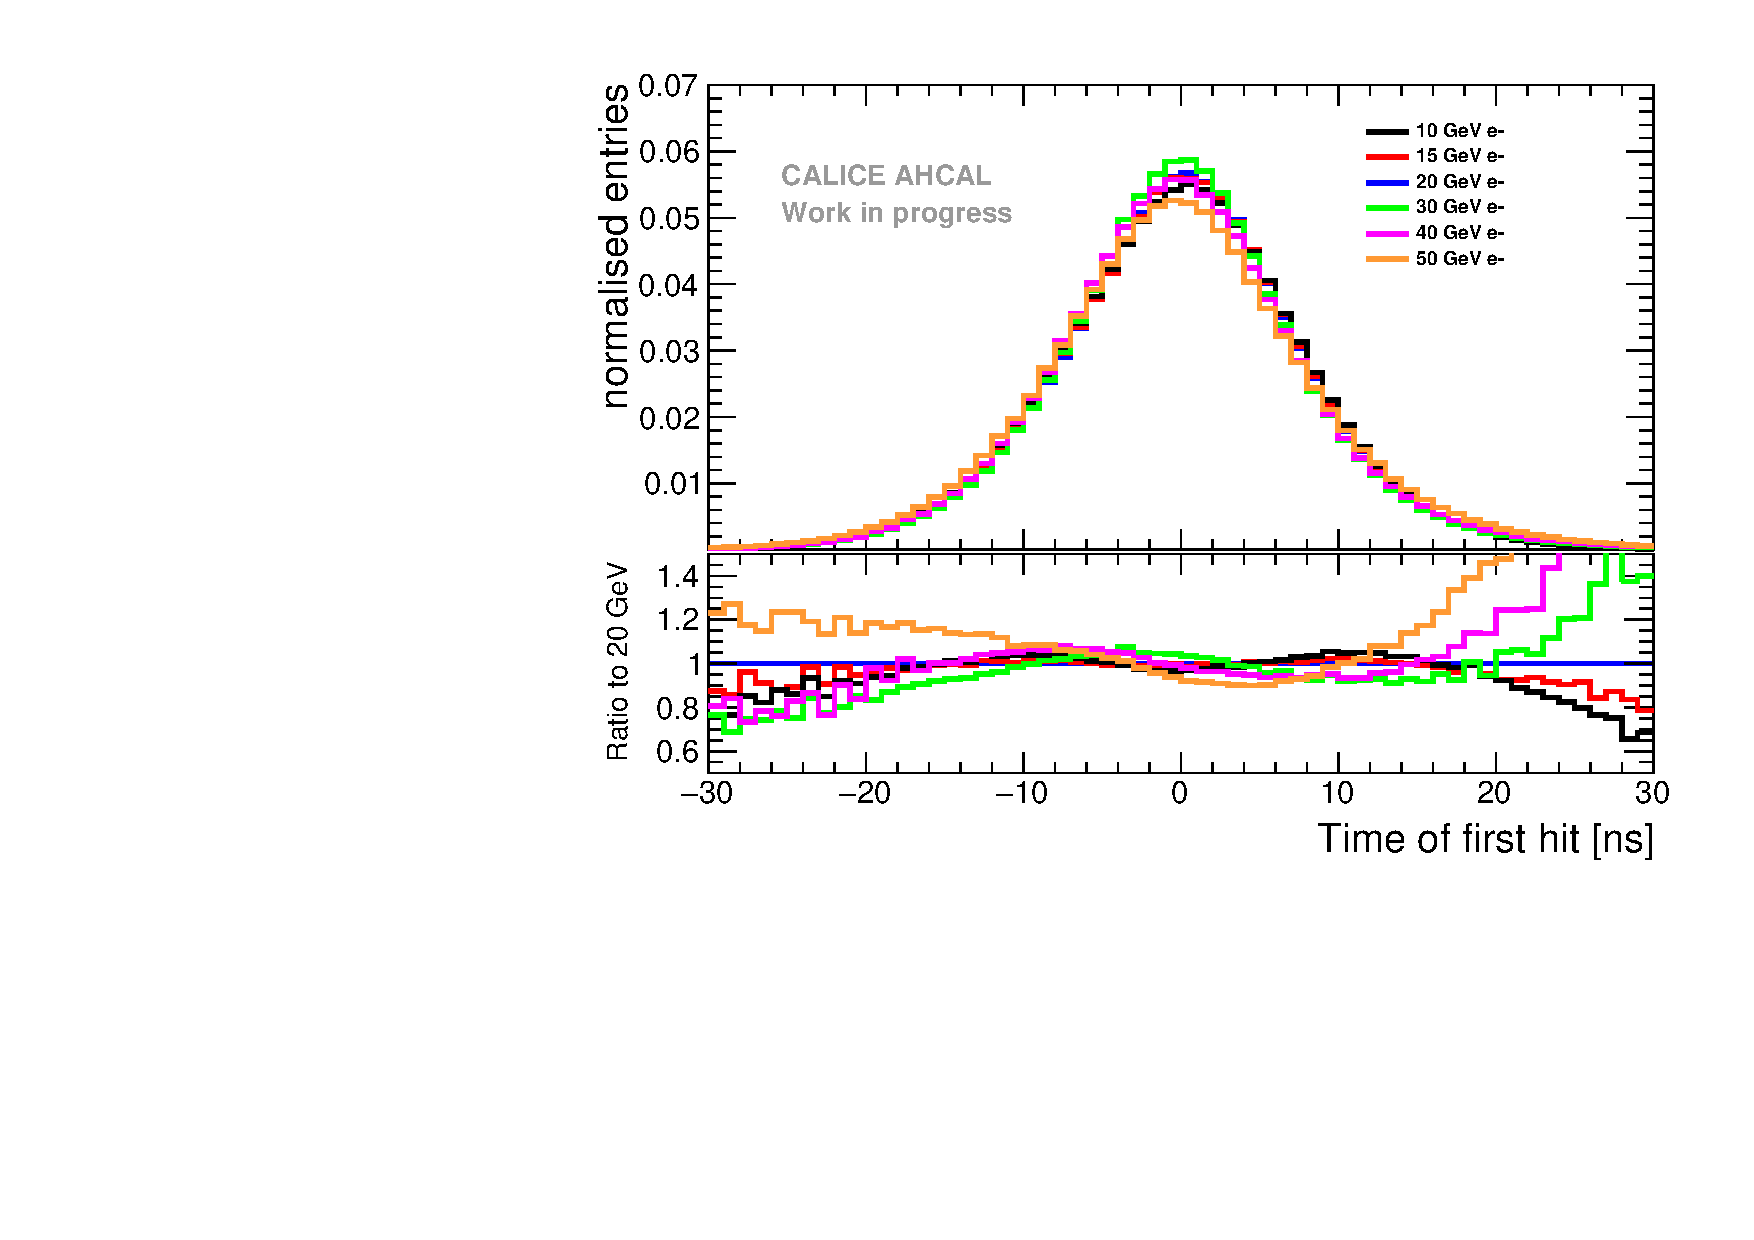
\includegraphics[width=0.6\textwidth]{../Thesis_Plots/Timing/Electrons/Plots/ComparisonDataEnergies.pdf}
	\caption{Comparison of the time of first hit distribution for all electron energies.}
	\label{fig:all_electron_energies}
\end{figure}

All electron runs (see section \ref{sec:TimingIntro}) have been carefully checked to validate the correction and the timing calibration. The figure \ref{fig:all_electron_energies} shows the comparison from 10 GeV to 50 GeV. The time distributions are in good agreement for all energies. The mean of the time distributions is very similar for all energies. The RMS of the time distributions varies between 7.86 ns at 10 GeV and 8.50 ns at 50 GeV corresponding to an increase of 8.1\%.

\section{Influence of the detector inhomogeneity}
\label{subsec:det_inhomo}

A study has been performed to estimate the influence of the detector inhomogeneity in space on timing. For this, only events in which the center of gravity in x and y is within the four center tiles of the detector are selected. Each of the four tiles is study separately. This has been performed for 10 and 50 GeV electron beam energy. The difference between the distributions helps to estimate the systematic uncertainty due to the inhomogeneity of the detector to which electrons are very sensitive to.

\begin{figure}[htbp!]
	\begin{subfigure}[t]{0.5\textwidth}
		\centering
		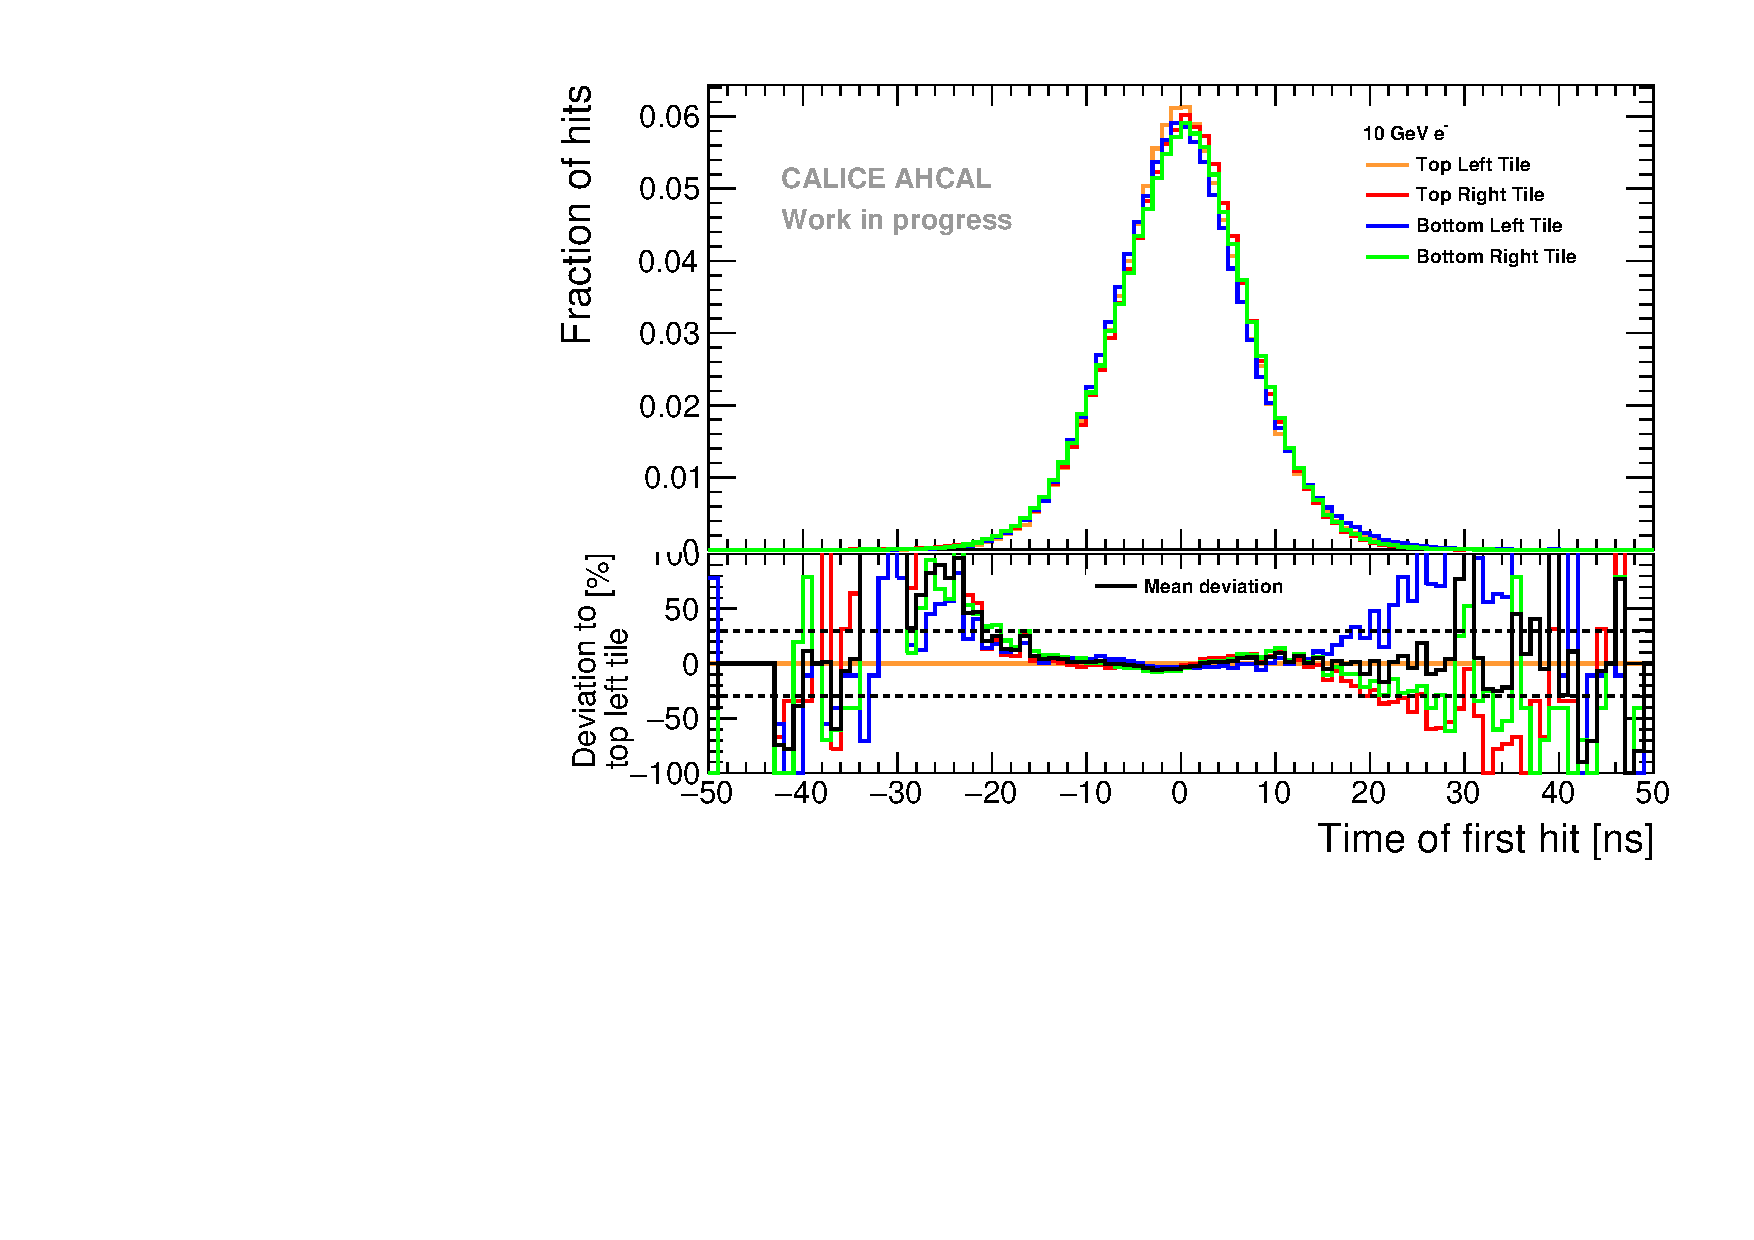
\includegraphics[width=1\textwidth]{../Thesis_Plots/Timing/Electrons/Plots/Systematic_Inhomogeneity_10GeV.pdf}
		\caption{}\label{fig:timing_inhomo_10GeV}
	\end{subfigure}
	\hfill
	\begin{subfigure}[t]{0.5\textwidth}
		\centering
		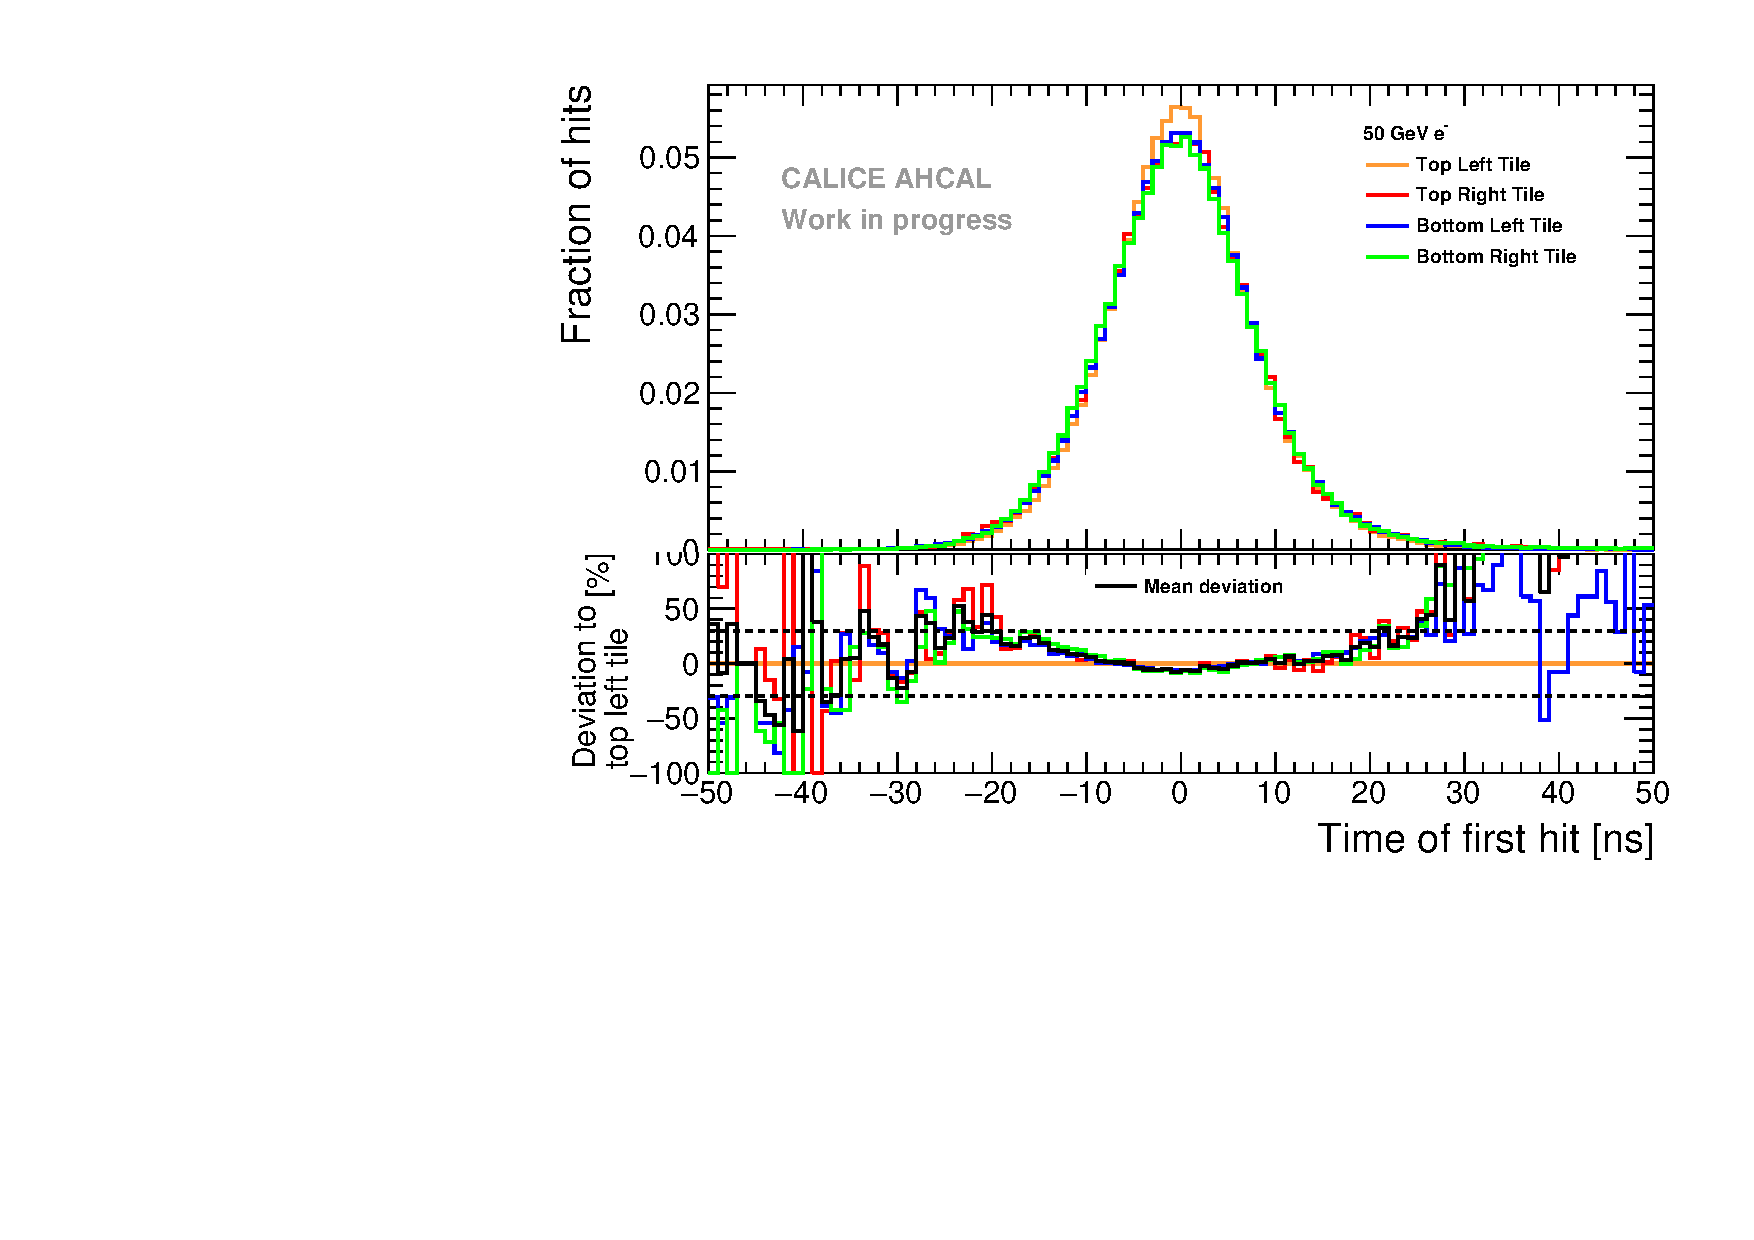
\includegraphics[width=1\textwidth]{../Thesis_Plots/Timing/Electrons/Plots/Systematic_Inhomogeneity_50GeV.pdf}
		\caption{}\label{fig:timing_inhomo_50GeV}
	\end{subfigure}
	\caption{\subref{fig:timing_inhomo_10GeV}) Time of the first hit distribution for all four middle tiles with 10 GeV electron beam. \subref{fig:timing_inhomo_50GeV}) Time of the first hit distribution for all four middle tiles with 50 GeV electron beam. All distribution are within 10-20\% in the core.}
\end{figure}

The figures \ref{fig:timing_inhomo_10GeV} and \ref{fig:timing_inhomo_50GeV} show the time distribution for each of the four tiles at 10 and 50 GeV respectively. The ratio shown is compared to the top left center tile. At 50 GeV, the mean of the distributions vary between -0.02 ns and -0.13 ns. The RMS of the distributions vary between 7.86 ns and 8.33 ns corresponding to an increase of 6\%. For both energies, the distributions are within a 10-20\% agreement in the region between -20 ns and 20 ns. Therefore a conservative systematic uncertainty of 20\% is assigned to electron and pion data in the following.

\section{Transportability of the calibration}

A check on the validity of the calibration for other data-taking periods has been performed on another dataset from a testbeam at DESY II in May 2016. The goal was to understand how transportable is the time calibration. The setup was composed of the same four big layers used at CERN in July 2015. In order to have enough hits in all layers, an aluminum absorber of 3 $X_{0}$ was placed in front of the detector in a 3 GeV electron beam.

\begin{figure}[htbp!]
	\centering
	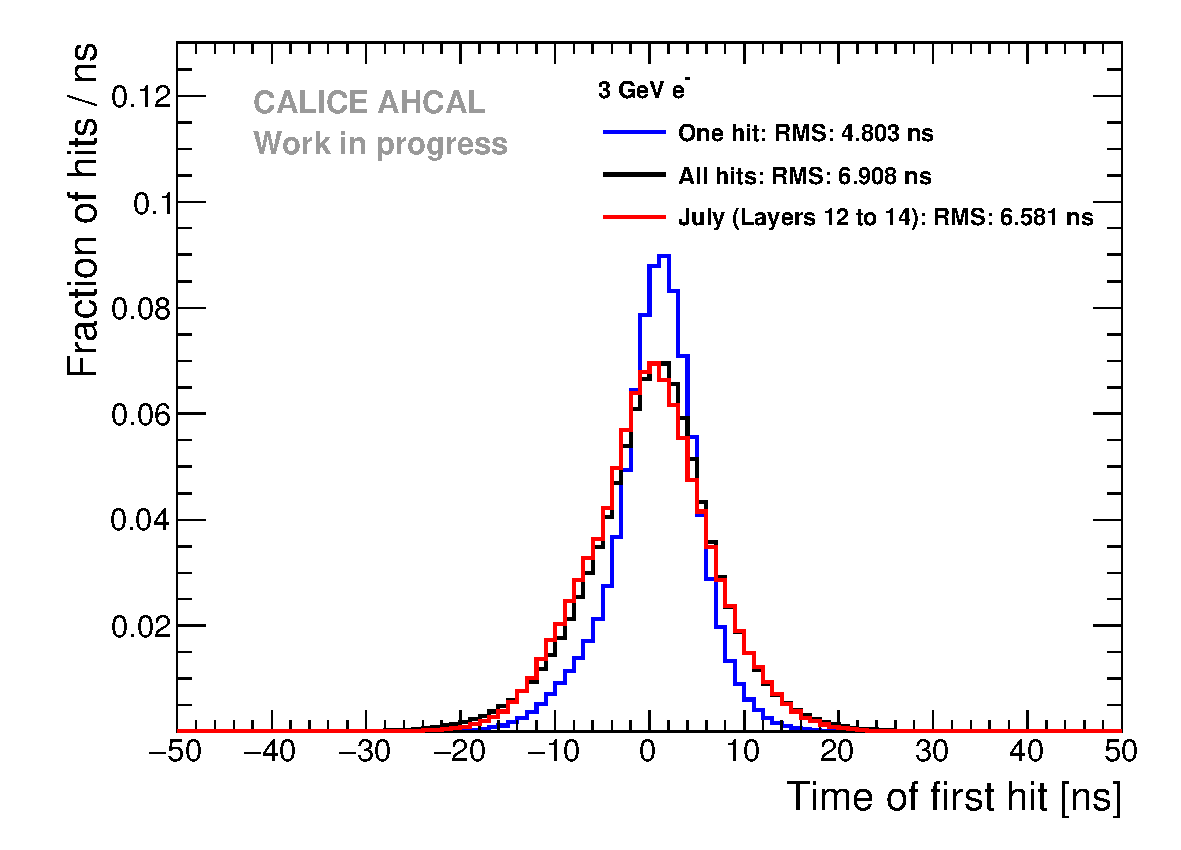
\includegraphics[width=0.6\textwidth]{../Thesis_Plots/Timing/Electrons/Plots/Timing_May2016_BigLayers.pdf}
	\caption{Time of the first hit distribution for 3 GeV electron showers at the DESY II testbeam in May 2016 combining layer 13 and 14.}\label{fig:TBMay2016}
\end{figure}

The same calibration constants determined from the CERN muon and electron data were used. Just a re-calibration of the time reference triggers ($T_{0}$) and the trigger time offset was necessary as the setup was different (different cabling and trigger logic).

The figure \ref{fig:TBMay2016} shows the distribution of the time of first hits for layer 13 and 14. The time resolution obtained of 7 ns is slightly better than the time resolution obtained at CERN in July 2015. The time distribution is narrower compared to the time distribution obtained at CERN. This is due to a lower number of hits per chip related to a lower beam energy. Thus the width of the distribution is smaller with the effect observed in section \ref{subsec:ped_shift}.

We can learn from this study, that the time calibration constants determined in a specific dataset can also be used for another dataset with the same layers. Therefore, the timing calibration depends mainly on hardware and not so much on the environment.

\section{Systematic uncertainties}

For a significant assessment of differences observed between data and simulations, systematic uncertainties must be evaluated. Several possible sources were identified:

\begin{itemize}
	\item Non-Linearity correction: A non-linearity correction, as explained in section \ref{subsec:lin_corr}, determined from data with a limited accuracy lead to a systematic uncertainty. The residuals of the correction give a systematic error at the level of 0.2 ns.
	\item Time walk correction: Similarly to the non-linearity correction, the systematic error obtained from the residuals of the time walk correction (see section \ref{subsec:timewalk}) is in the order of 0.2 ns.
	\item Number of triggered channels correction: The correction for the number of triggered channels over 0.5 MIP in a chip results in a residual on the timing in the order of 1 ns. This systematic error is the most dominant over all other uncertainties.
	\item Time smearing parametrization: A parametrization was obtained from data for the width of the time smearing as a function of the number of triggered channels. An error band was obtained by comparing all electron energies as explained in appendix \ref{appendix:ped_shift}. This is applied to simulation for systematics.
	\item Determination of the offset to $t=0$: For simulation, the time shift per layer is calculated using a time of flight correction $T_{of} = \frac{z_{layer}}{c}$ with $c$ the speed of light and $z_{layer}$ the z position of a layer. For this, an uncertainty of 3 mm corresponding to the scintillator thickness is taken in z corresponding to 0.01 ns uncertainty in timing.
	\item Position of the detector relative to the beam: The detector was positioned in a way that the beam hits mostly the centered tiles. The uncertainty of the position of the layers is at the millimeter level. Thus a conservative uncertainty of a tile (3 cm) is taken. This uncertainty converted to time using QGSP\_BERT\_HP varies between 0.36 ns at $r = 1.5$ cm to 1.27 ns at $r = 19.5$ cm for the layers 1 to 10 and between 0.15 ns at $r = 1.5$ cm to 0.67 ns at $r = 31.5$ cm for the layer 11 to 14 with 10 GeV pion beam energy.
	\item Cross-talk: No measurement for optical cross-talk between tiles is available and from previous measurements, it varies between 10\% and 18\%. These are used for systematics in simulation only for the layers 4 to 10. The cross-talk value induces a different number of hits in the detector thus has an impact on the width of the time distribution.
	\item Detector inhomogeneities: As explained in section \ref{subsec:det_inhomo}, variations in the absolute number of entries in each time bins can be observed. The variations are between 10-20\% thus a conservative error of 20\% is used for the time distribution.
	\item Absolute number of events: In the pion data, some possible contamination from multi-particle events may be present still after the selection as shown in section \ref{sec:pionsel}. Thus the number of absolute pion events is not known. A conservative error of 10\% is taken into account when comparing data to simulation for the absolute number of hits per time bin.
\end{itemize}

The systematic uncertainties are added in quadrature for the full systematic uncertainty. For comparison between data and simulation of the absolute time distribution, this results in an uncertainty of 20\% for muons/electrons and 30\% for pions is used. For the mean time of the first hit as a function of the hit energy, the systematic uncertainty is resulting at 1.04 ns. For the mean time of first hit as a function of the hit distance to the shower center of gravity, the systematic uncertainty is varying between 0.36 ns at small radius to 1.54 ns at large radius for the layers 1 to 11 and from 0.15 ns at small radius to 0.95 ns at large radius for the layers 11 to 14. The table \ref{table:time_syst} sums up the systematic uncertainties used in the analysis.
%% Systematics from number of hits may be underestimated... %
{
\renewcommand{\arraystretch}{1.2}
\begin{table}[htb!]
	\centering
	\caption{Summary of systematic uncertainties.}
	\label{table:time_syst}
	\begin{tabular}{@{} lc @{}}
		\toprule
		\multicolumn{1}{c}{Uncertainty source} & Full uncertainty steel \\
		\midrule
		% MIP Energy Scale & XXX-XXX ns \\
		Non-linearity residuals & 0.2 ns \\
		Time-walk residuals & 0.2 ns \\
		Number of triggered channels residuals & 1 ns \\
		Offset to $t=0$ & 0.01 ns (MC) \\
		Position relative to the beam & 0.36-1.54 ns (Layers 1 to 10) / 0.15-0.95 ns (Layer 11 to 14) \\
		Cross-talk & 10-18\% \\
		Detector inhomogeneities & 20\% \\
		Number of absolute events & 10\% (pions) \\
		\midrule
		\midrule
		\multicolumn{2}{c}{Systematics combined} \\
		\midrule
		data-MC hits per time bin & 20\% (muons/electrons) - 30\% (pions) \\
		data-MC vs hit energy & 1.04 ns \\
		data-MC vs hit distance to CoG & 1.10-1.86 ns (Layers 1 to 10) / 1.05-1.41 ns (Layer 11 to 14) \\
		\bottomrule
	\end{tabular}
\end{table}
}

\section{Validation of the simulation}

The simulation is validated by comparing the recorded muon and electron data to simulations. The timing resolution is extracted from muon data runs by fitting a double Gaussian to the data in the range [-50 ns, 50 ns] and is used to smear the timing of simulated calorimeter hits. The table \ref{table:time_res_sim} sums up the parameters used.

\begin{table}[htb!]
	\centering
	\caption{Timing resolution extracted with a double Gaussian fit from muon data used for simulation.}
	\label{table:time_res_sim}
	\begin{tabular}{@{} cccccc @{}}
		\hline
		$\alpha_{1}$ & $\mu_{1}$ [ns] & $\sigma_{1}$ [ns] & $\alpha_{2}$ & $\mu_{2}$ [ns] & $\sigma_{2}$ [ns] \\
		\hline
		0.607352 & -0.699093 & 5.85891 & 0.391041 & 0.945272 & 3.4012 \\
		\hline
	\end{tabular}
\end{table}

The comparison of the time of first hit distribution for muons is shown in figure \ref{fig:sim_data_muon}. The comparison shows that in the full range, the difference between data and simulation is around 10-20\% maximum. The large uncertainties observed in the simulation are due to the systematics of the different cross-talk values.

\begin{figure}[htbp!]
	\centering
	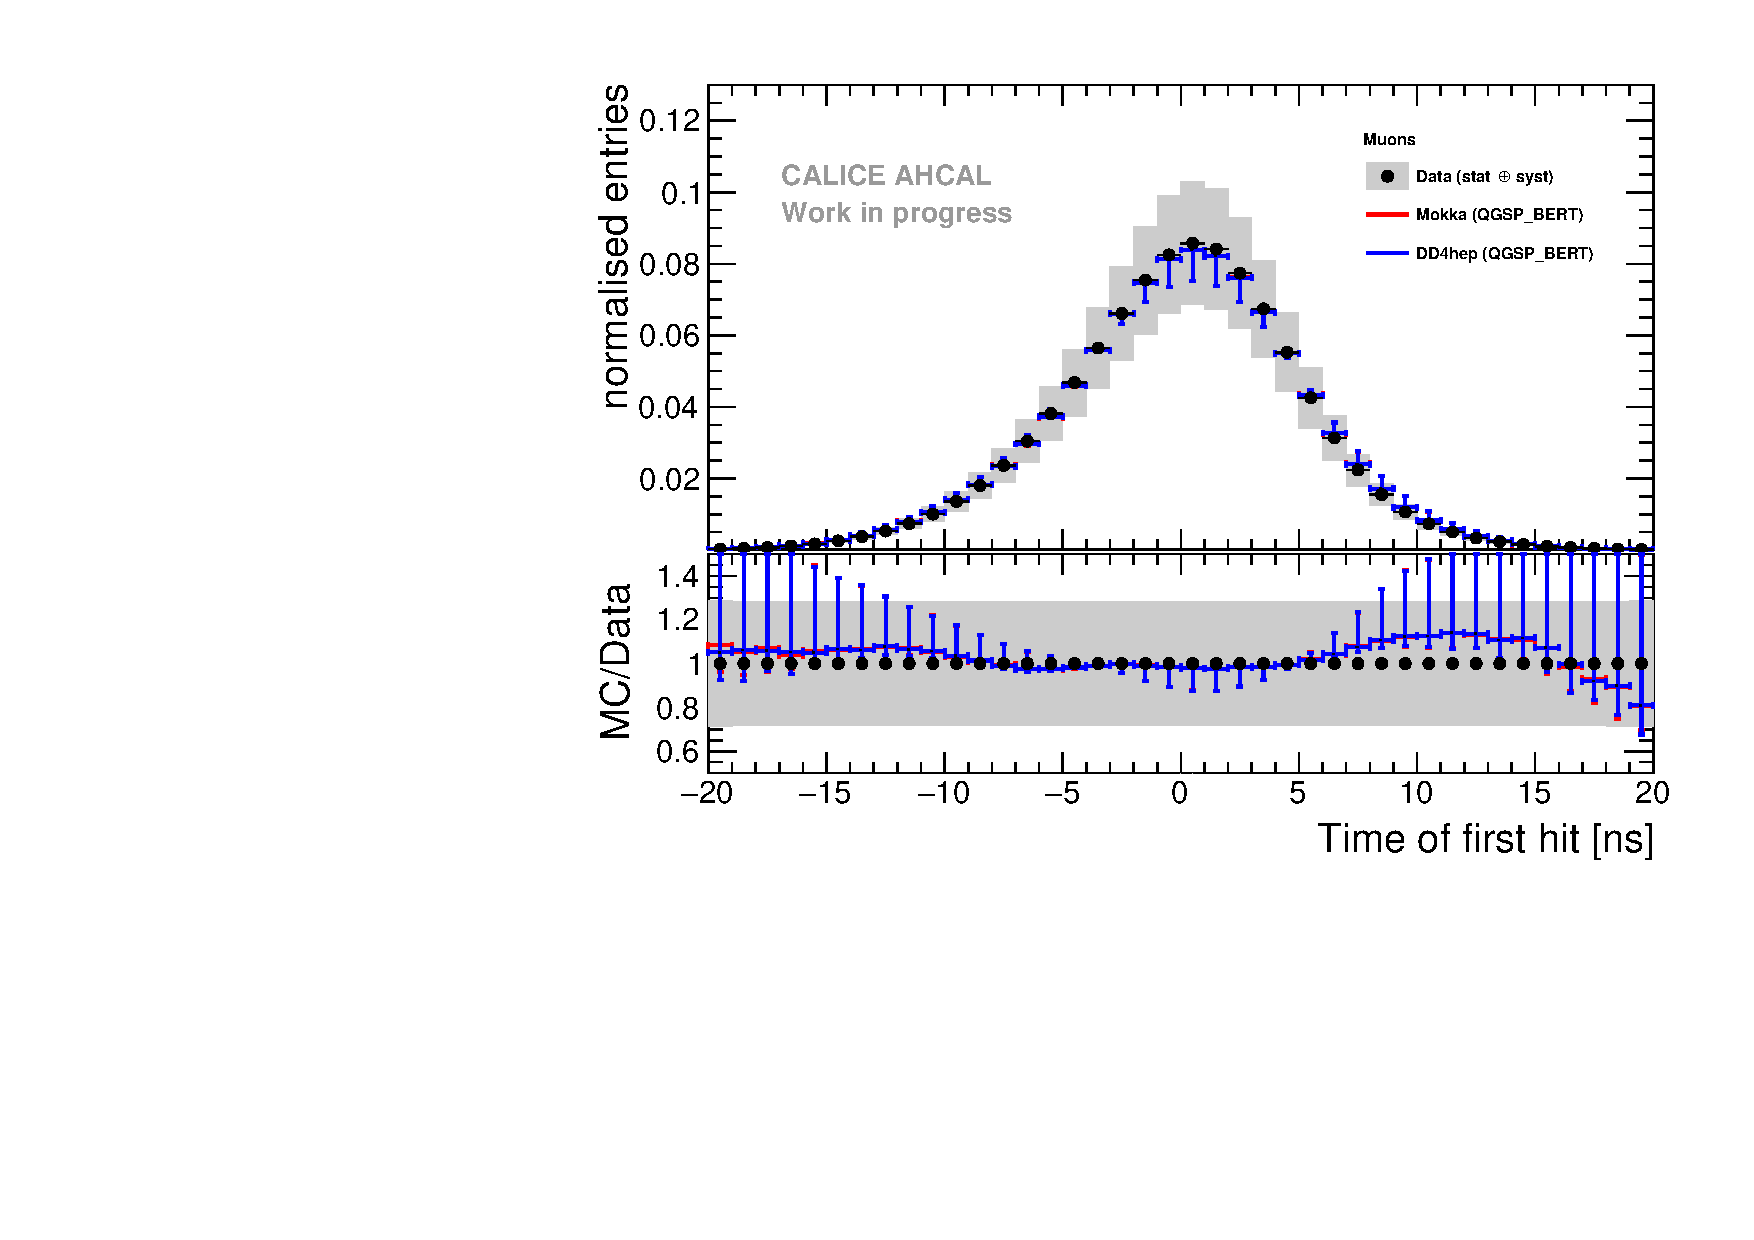
\includegraphics[width=0.6\textwidth]{../Thesis_Plots/Timing/Muons/Plots/Comparison_MokkaDD4hepData_Muons.pdf}
	\caption{Time of first hit for data and simulation between -20 and 20 ns.}
	\label{fig:sim_data_muon}
\end{figure}

In the next step, a comparison with electron data is necessary to validate the simulation. In addition to the muon resolution, a parametrization of the increase of the width of the time distribution as a function of the number of hits above 0.5 MIPs is added in simulation as described in appendix \ref{appendix:ped_shift}. Figure \ref{fig:sim_data_elec} shows this comparison.

\begin{figure}[htbp!]
	\begin{subfigure}[t]{0.5\textwidth}
		\centering
		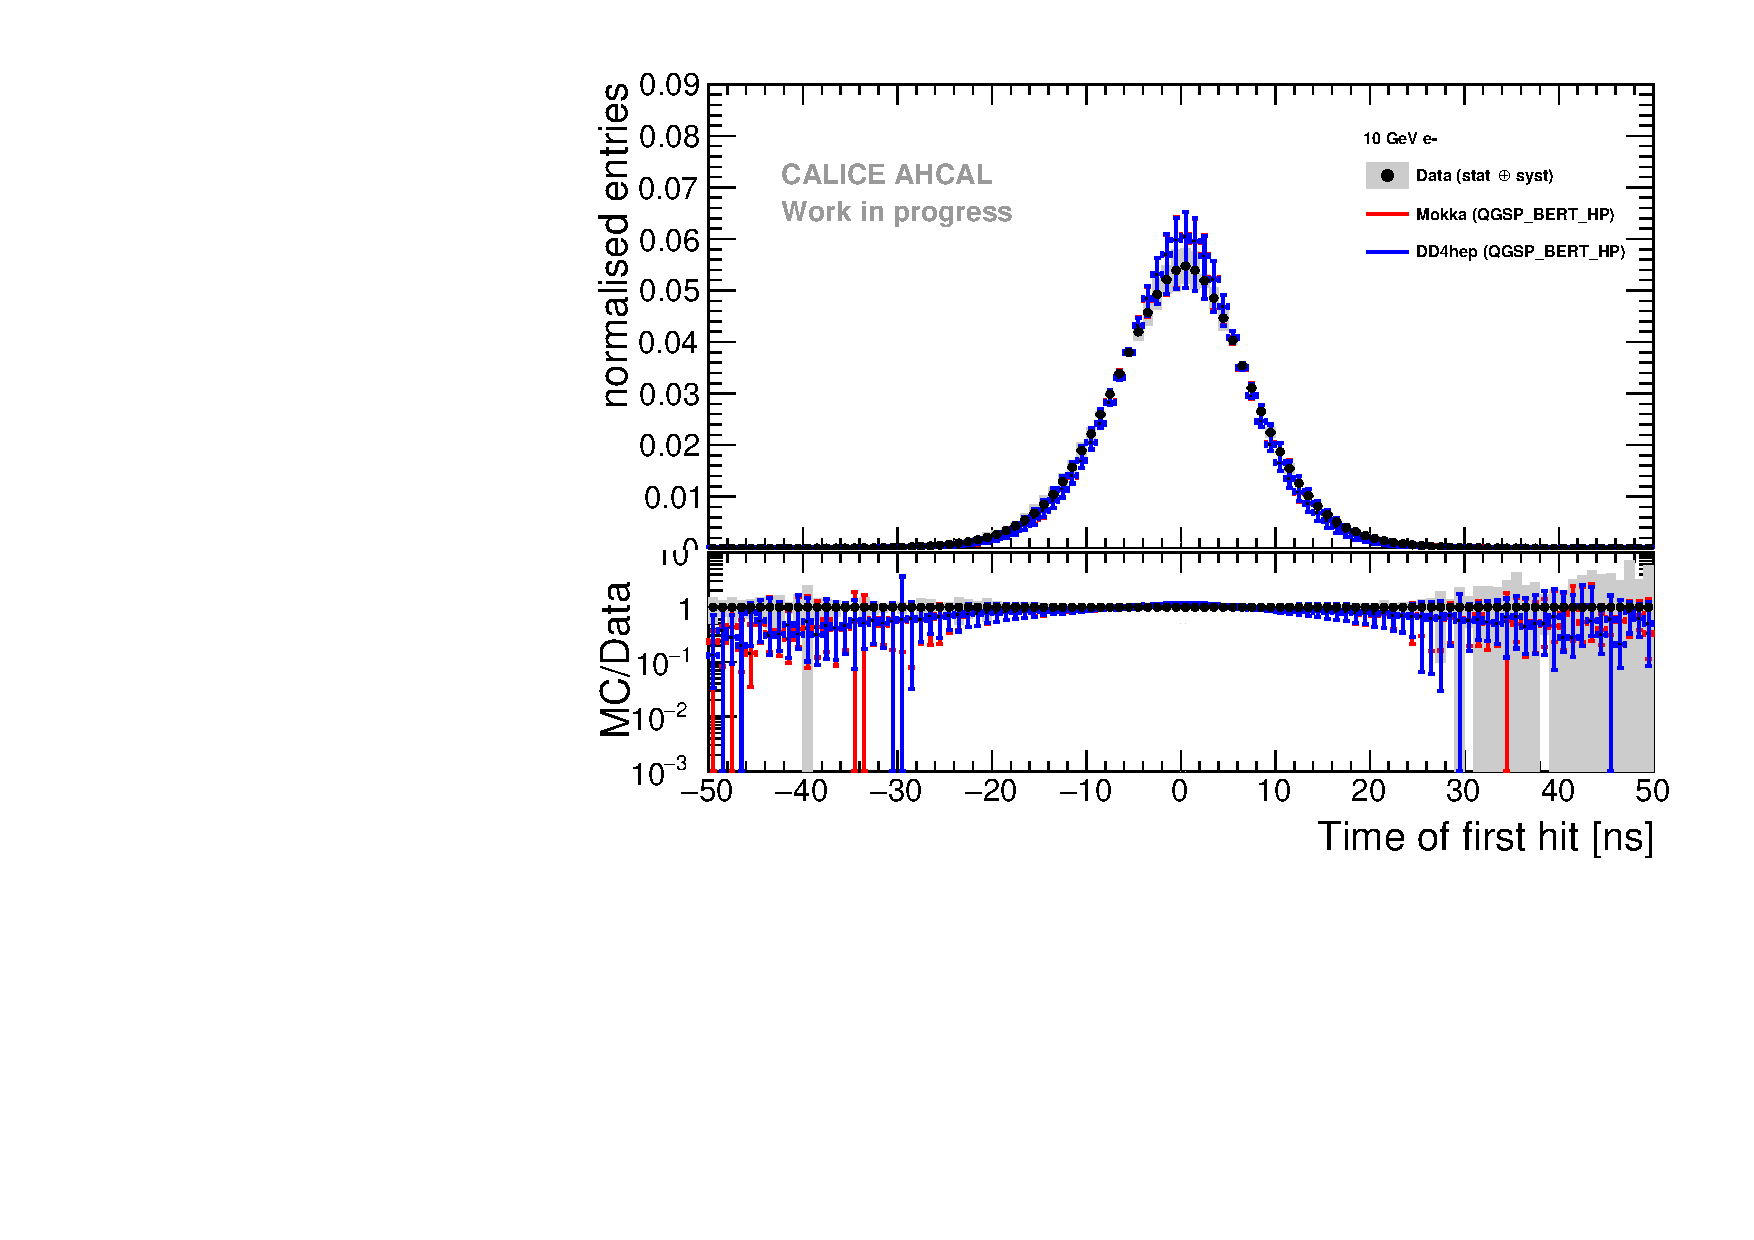
\includegraphics[width=1\textwidth]{../Thesis_Plots/Timing/Electrons/Plots/Comparison_SimData_Electrons10GeV.pdf}
		\caption{10 GeV.}\label{fig:elec_sim_data_10GeV}
	\end{subfigure}
	\hfill
	\begin{subfigure}[t]{0.5\textwidth}
		\centering
		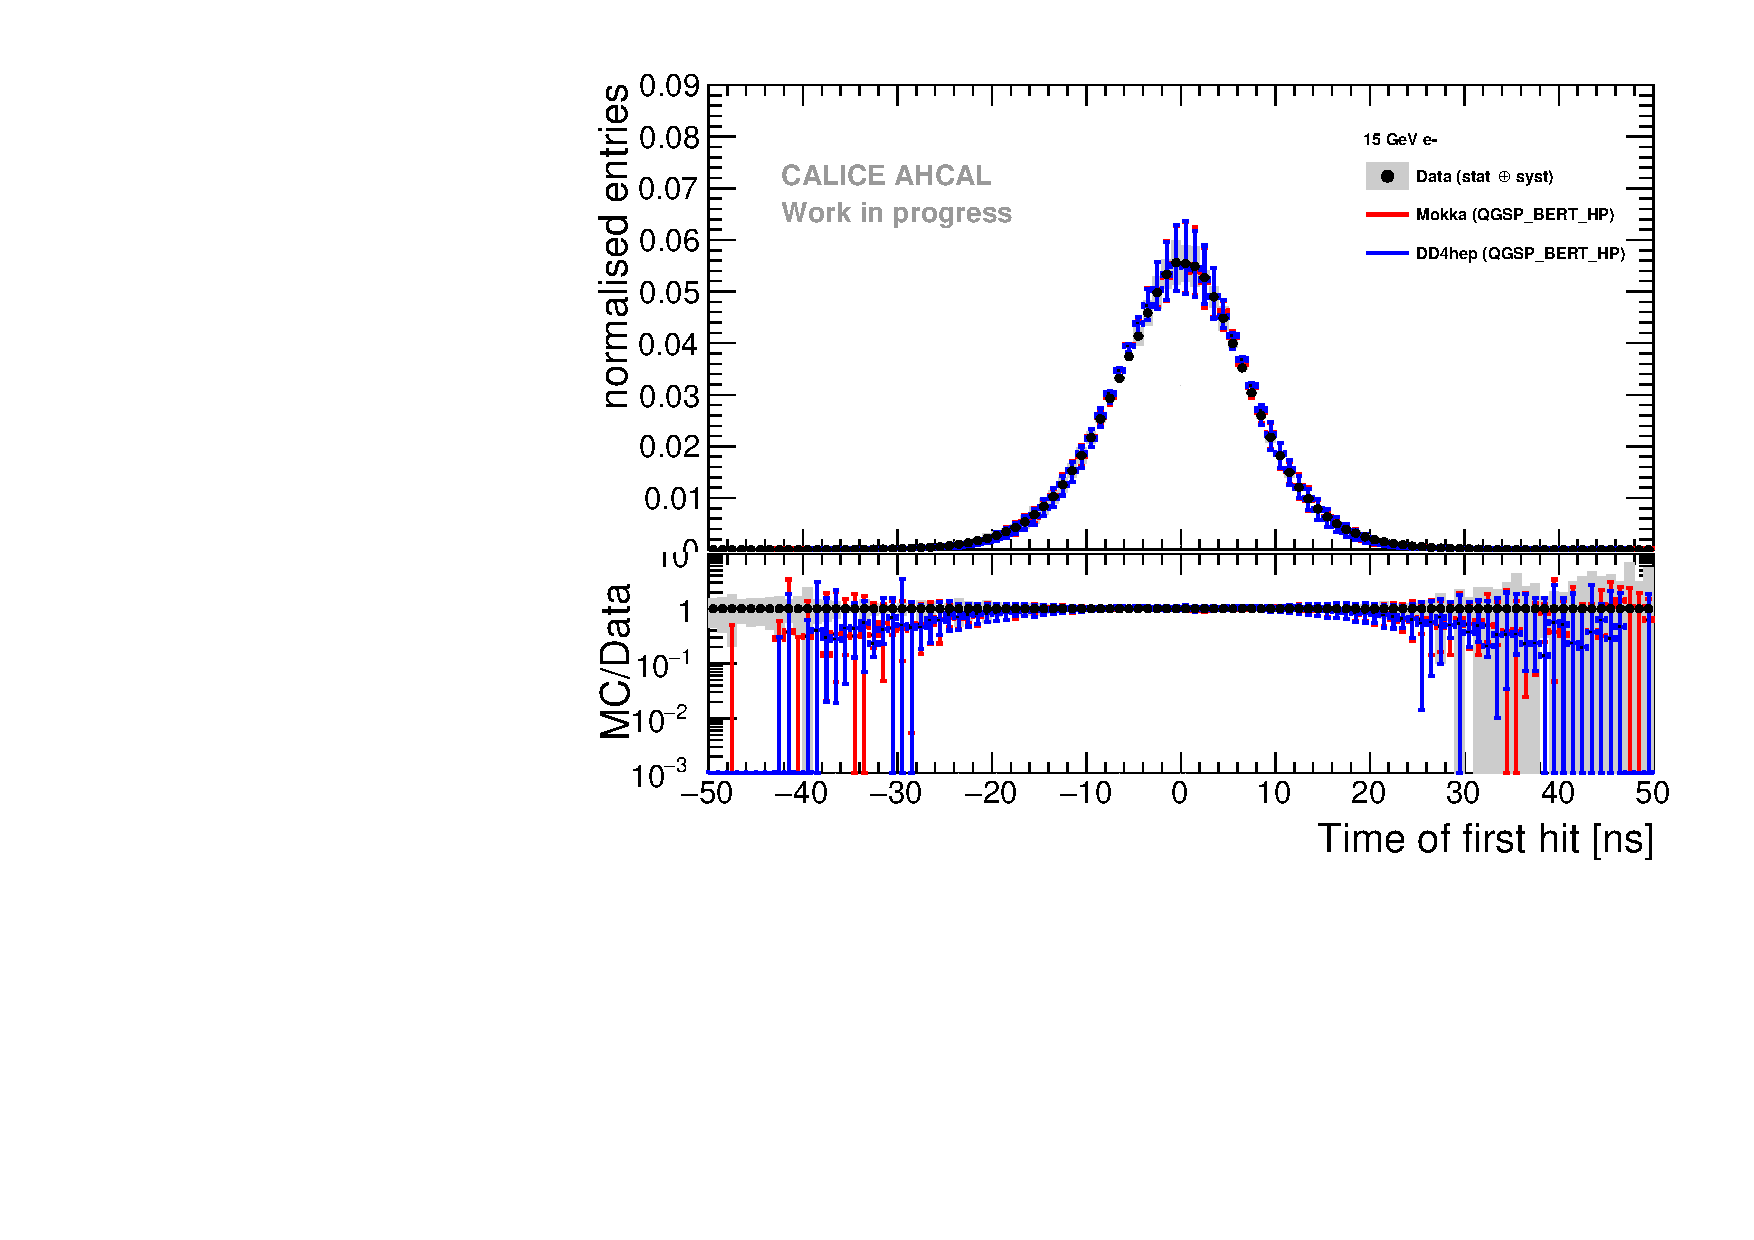
\includegraphics[width=1\textwidth]{../Thesis_Plots/Timing/Electrons/Plots/Comparison_SimData_Electrons15GeV.pdf}
		\caption{15 GeV.}\label{fig:elec_sim_data_15GeV}
	\end{subfigure}
	\hfill
	\begin{subfigure}[t]{0.5\textwidth}
		\centering
		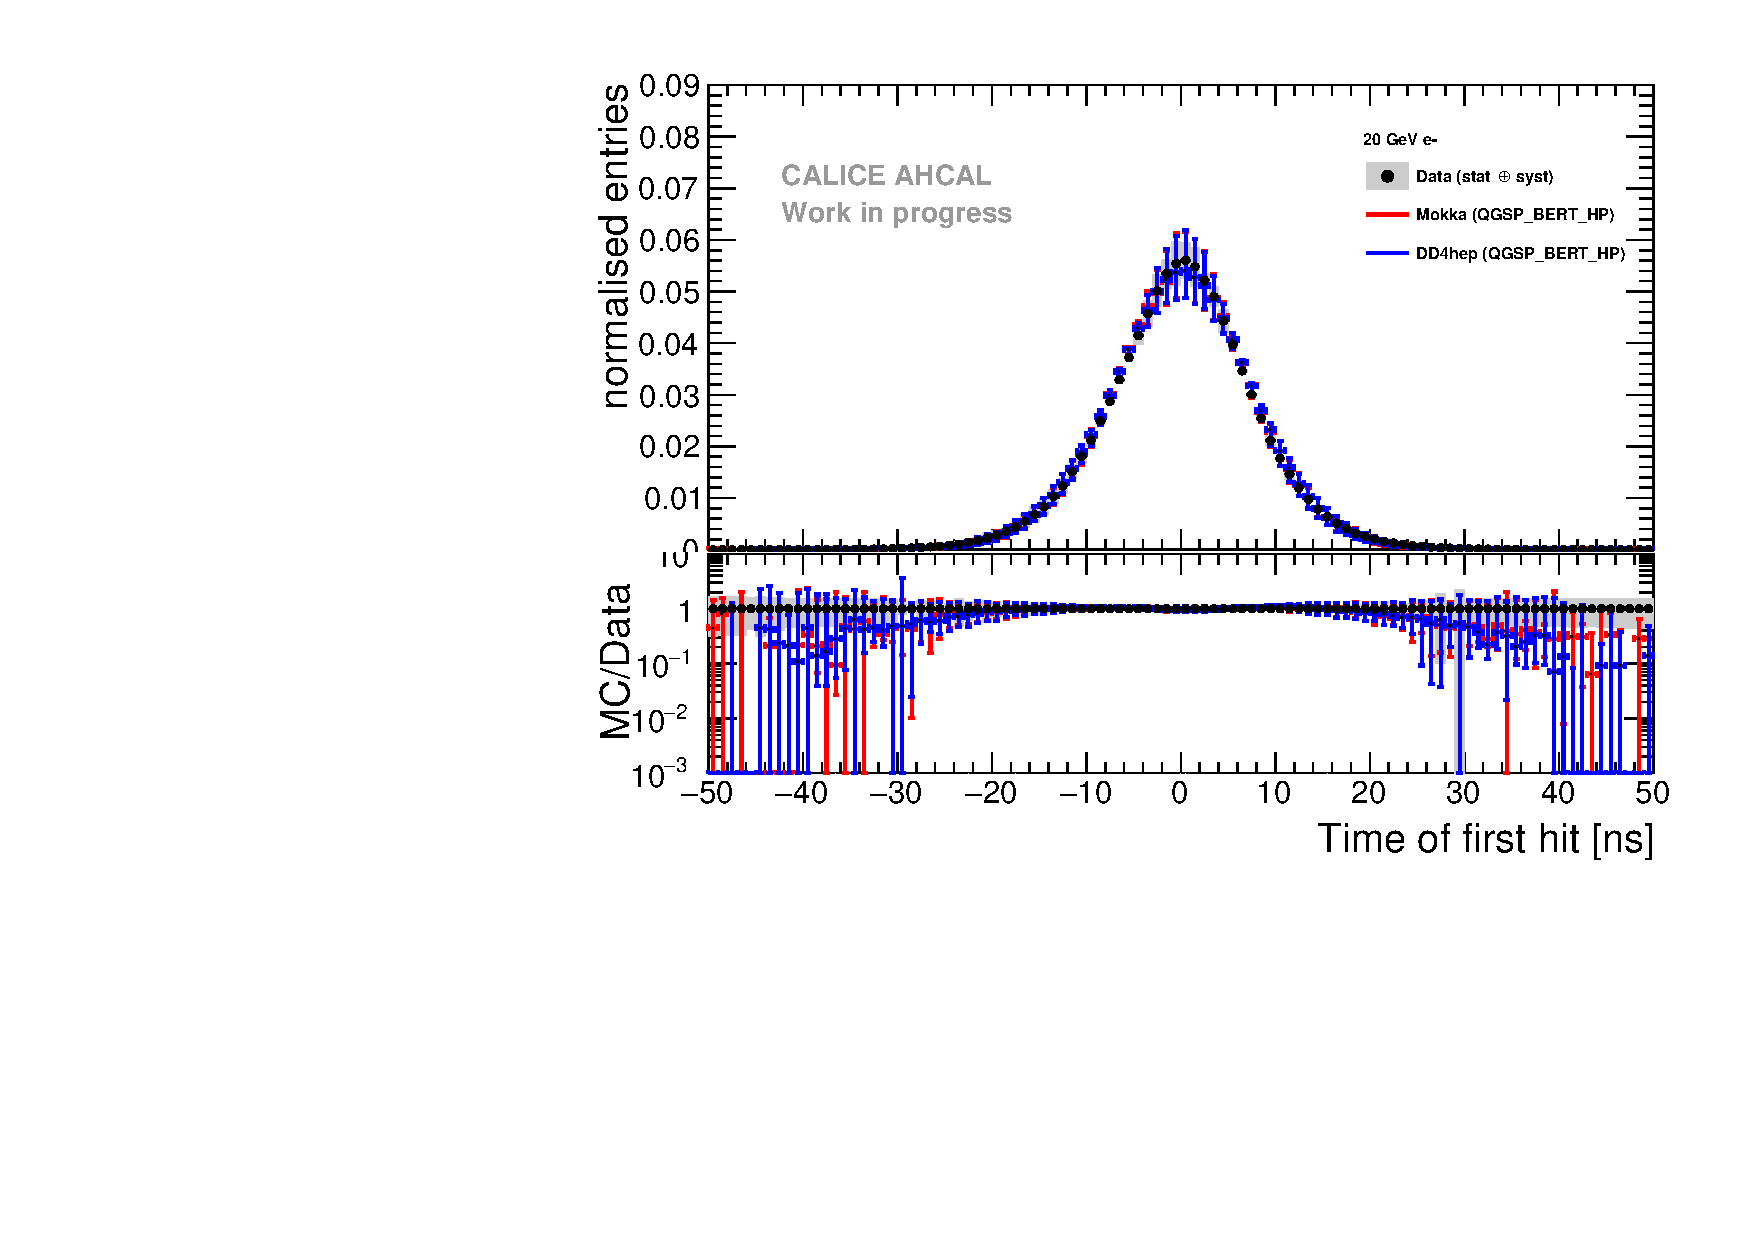
\includegraphics[width=1\textwidth]{../Thesis_Plots/Timing/Electrons/Plots/Comparison_SimData_Electrons20GeV.pdf}
		\caption{20 GeV.}\label{fig:elec_sim_data_20GeV}
	\end{subfigure}
	\hfill
	\begin{subfigure}[t]{0.5\textwidth}
		\centering
		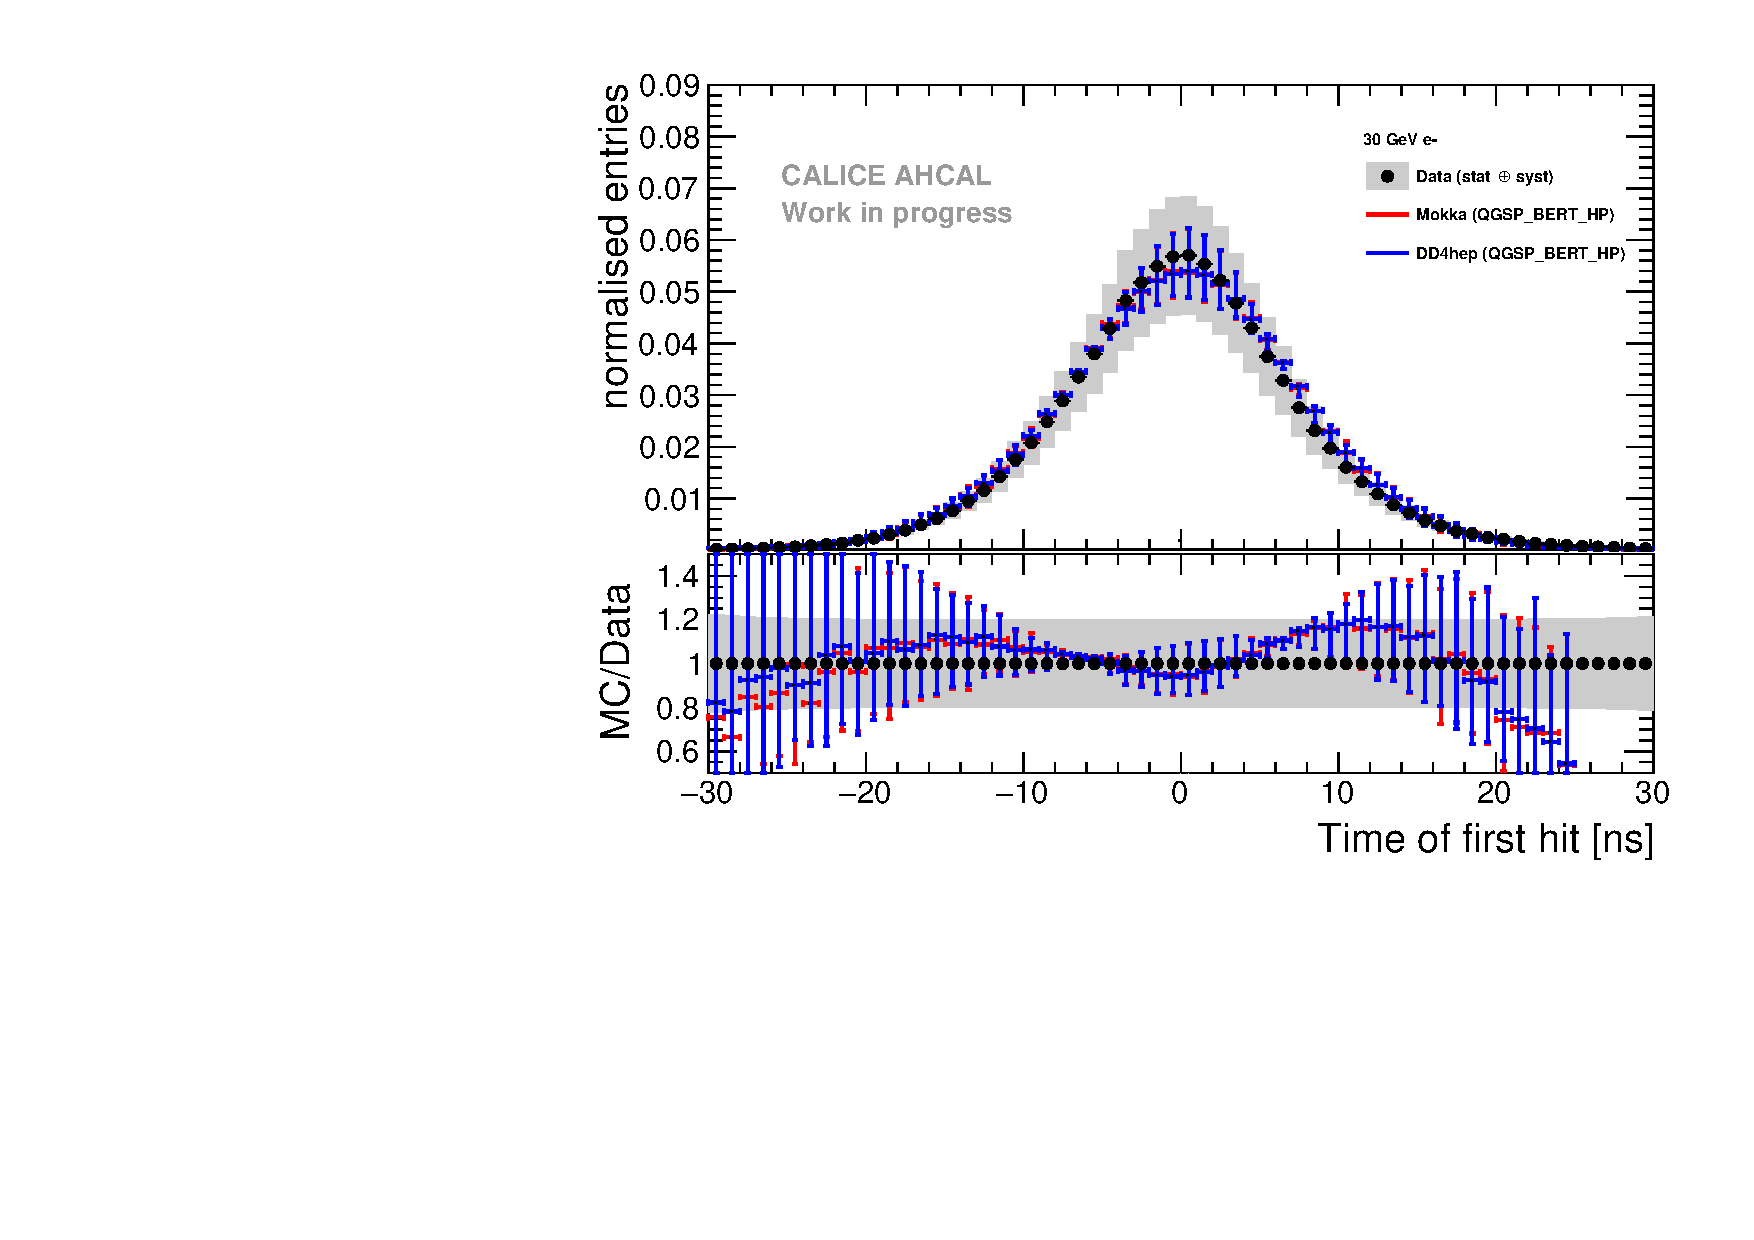
\includegraphics[width=1\textwidth]{../Thesis_Plots/Timing/Electrons/Plots/Comparison_SimData_Electrons30GeV.pdf}
		\caption{30 GeV.}\label{fig:elec_sim_data_30GeV}
	\end{subfigure}
	\hfill
	\begin{subfigure}[t]{0.5\textwidth}
		\centering
		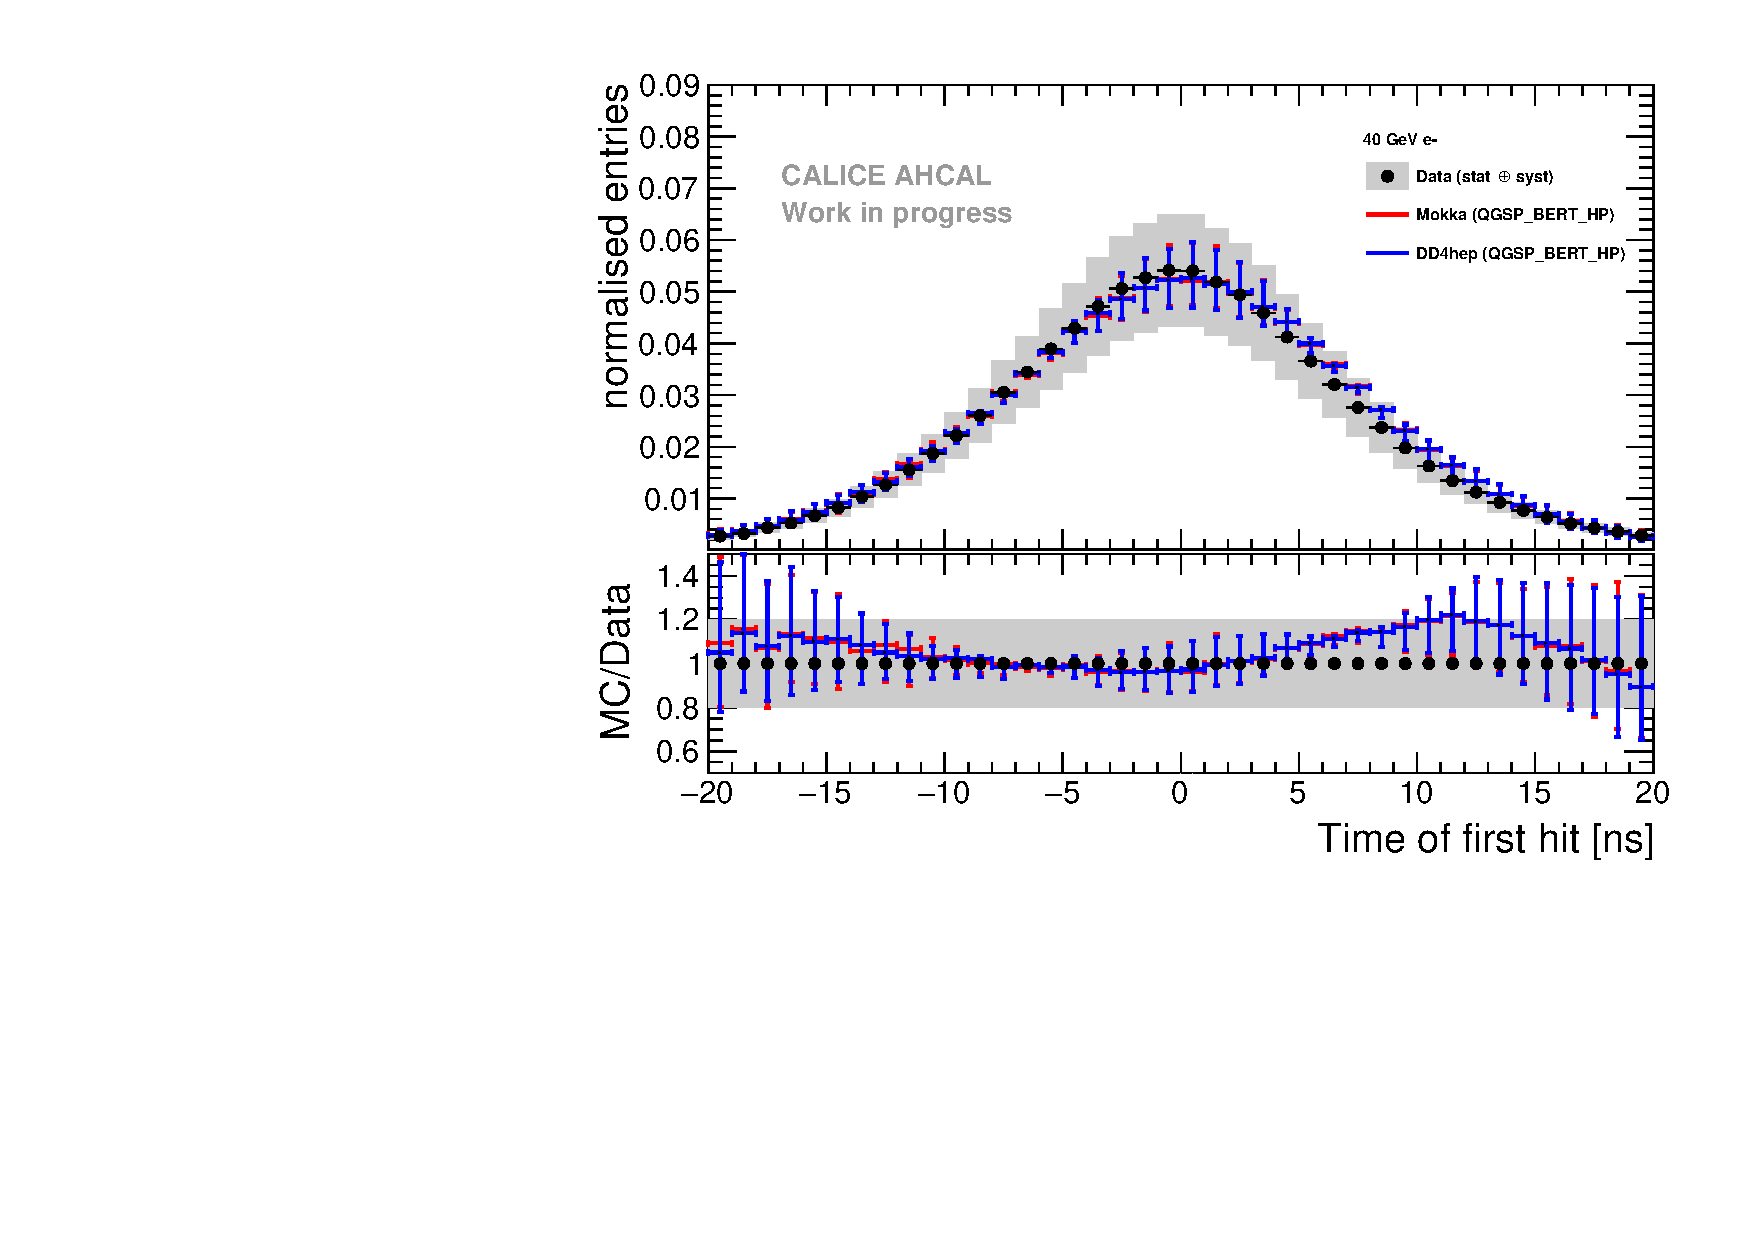
\includegraphics[width=1\textwidth]{../Thesis_Plots/Timing/Electrons/Plots/Comparison_SimData_Electrons40GeV.pdf}
		\caption{40 GeV.}\label{fig:elec_sim_data_40GeV}
	\end{subfigure}
	\hfill
	\begin{subfigure}[t]{0.5\textwidth}
		\centering
		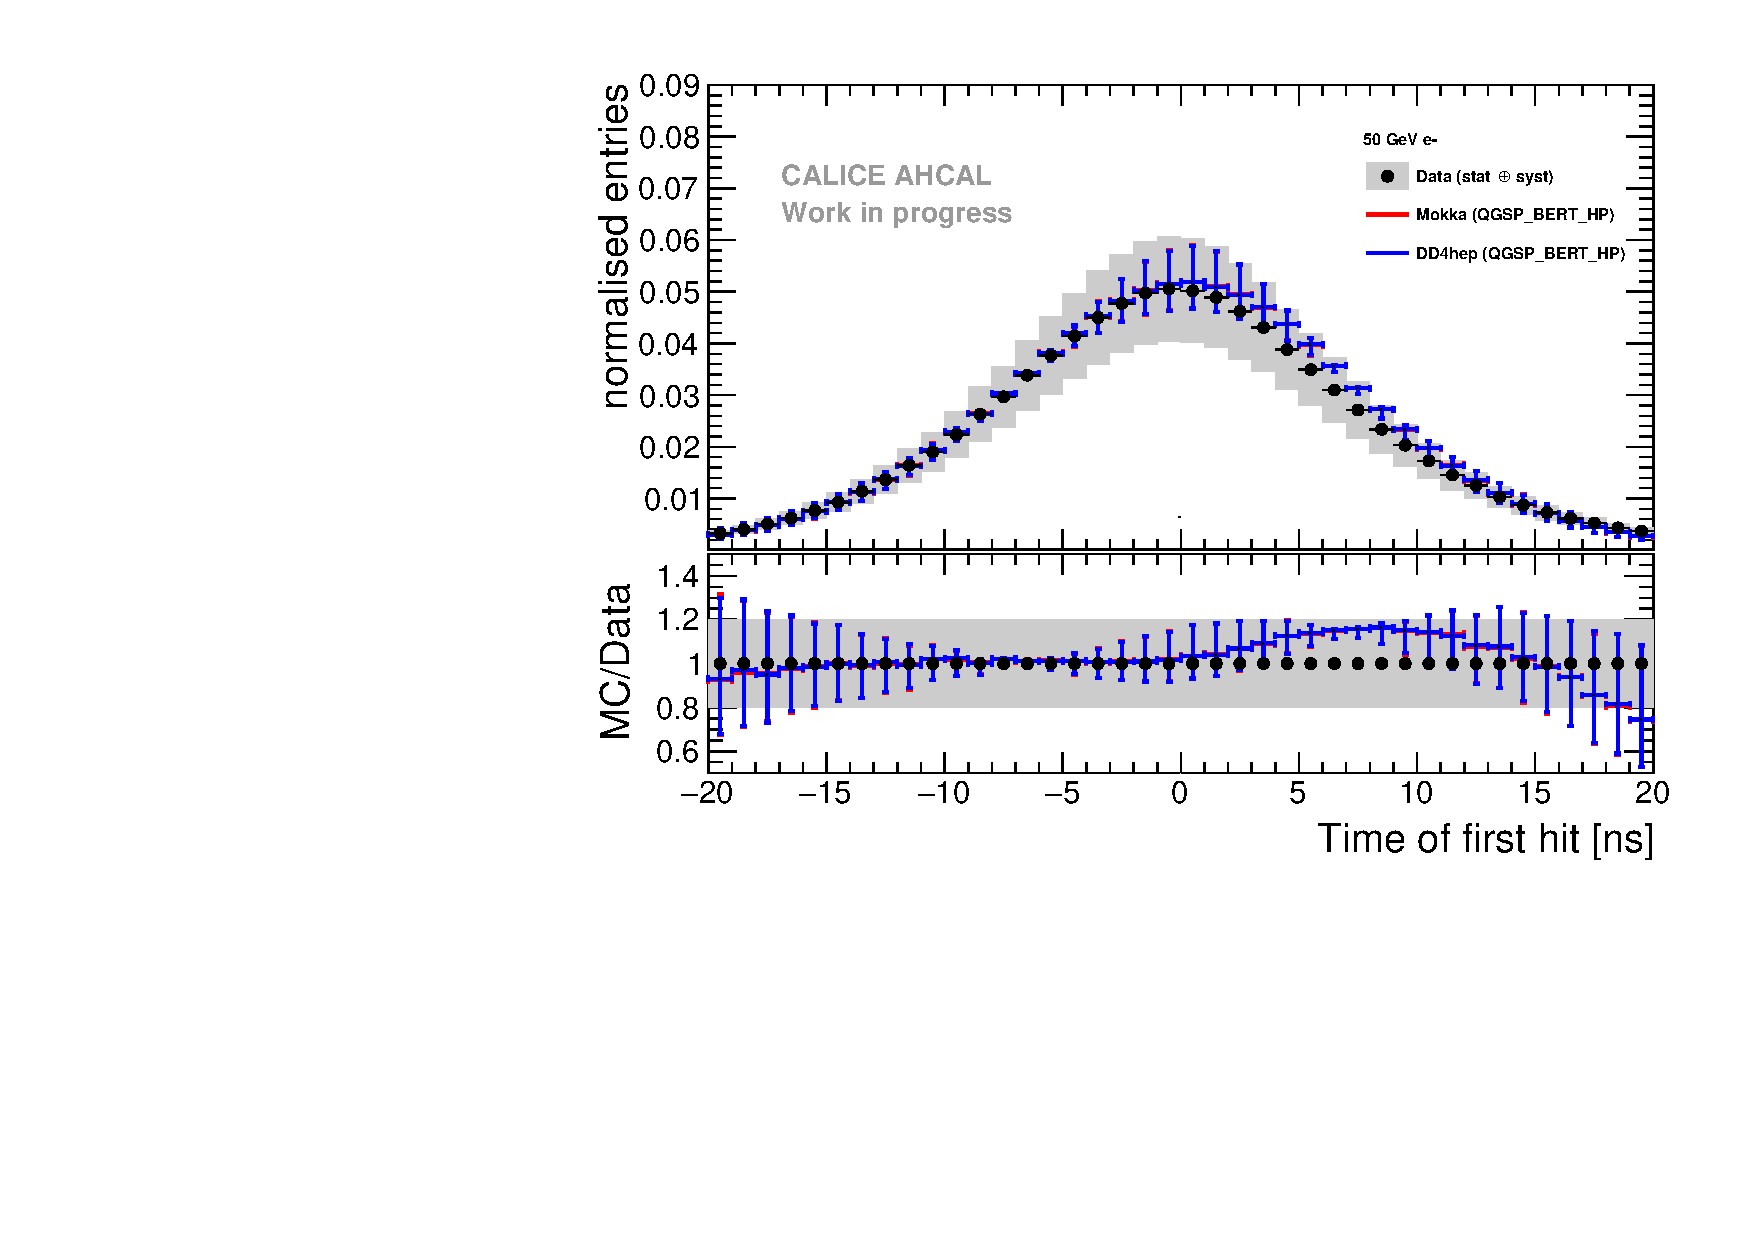
\includegraphics[width=1\textwidth]{../Thesis_Plots/Timing/Electrons/Plots/Comparison_SimData_Electrons50GeV.pdf}
		\caption{50 GeV.}\label{fig:elec_sim_data_50GeV}
	\end{subfigure}
	\caption{Comparison between electron data and MC for all energies of the time of first hit. The grey area represents the statistical and systematical error of the data. Error bars in simulation are obtained by varying the cross-talk parameter and with the error envelope from the number of hits parametrization.}
	\label{fig:sim_data_elec}
\end{figure}

The simulation is systematically narrower than data for all energies. This would suggest that simulation has fewer hits than data which is in agreement with figure \ref{fig:sim_data_elec_nHits}, where generally simulation is 10-20\% lower than data in the region of 6 to 10 hits per chip. For the time of first hit, The simulation is in better agreement for higher energies, at 40-50 GeV, than for lower energies at 10-15 GeV. This may come from imperfect beam profiles where a slight shift in the simulation can influence highly the number of triggers in a chip. Also, the number of triggered channels parametrization may be imperfect. But due to the limited amount of data, only a global parametrization could be applied. For 10 to 20 GeV comparisons, the description of the tails in the simulation that are quite underestimated. This may be due to the description of the noise in the simulation that is not perfectly reproduced. Overall, the simulation and data are in agreement within statistical and systematic uncertainties.

\begin{figure}[htbp!]
	\begin{subfigure}[t]{0.5\textwidth}
		\centering
		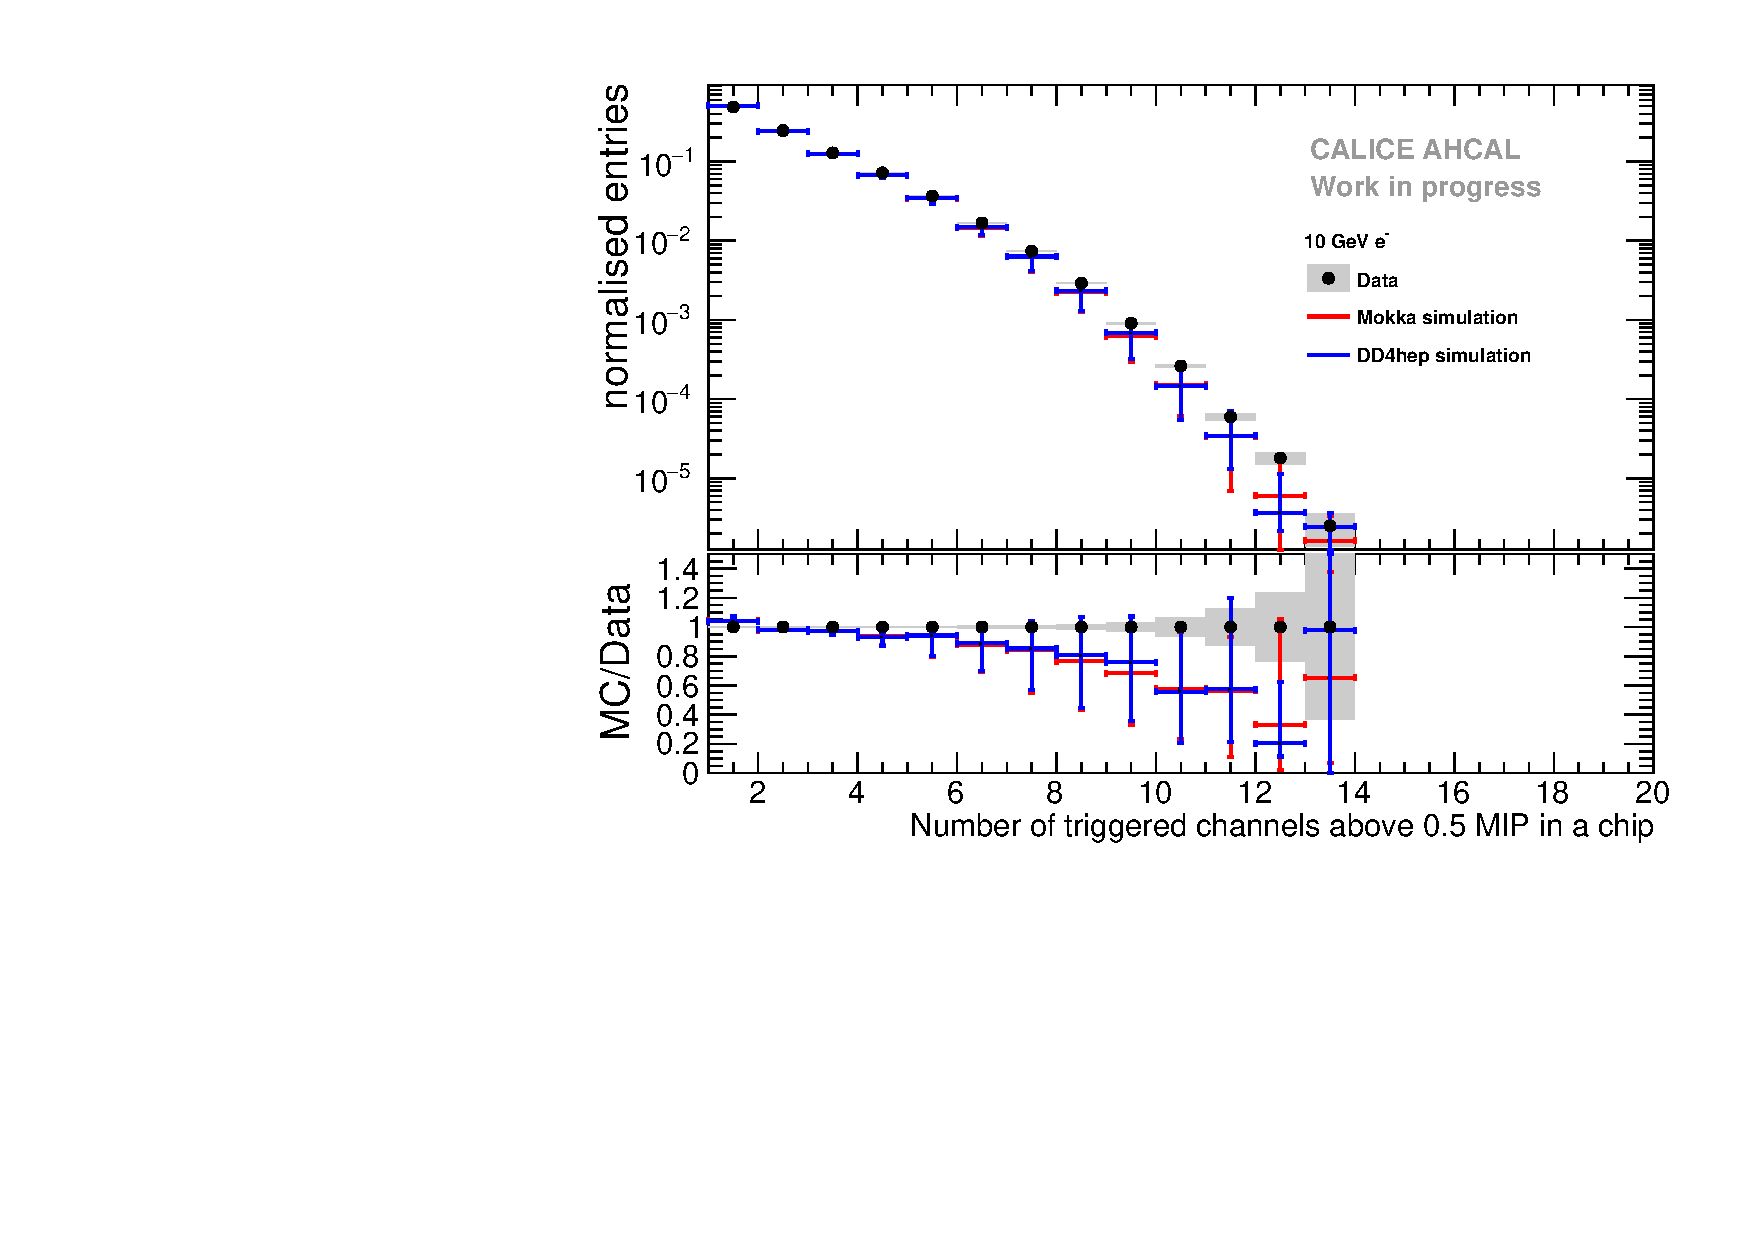
\includegraphics[width=1\textwidth]{../Thesis_Plots/Timing/Electrons/Plots/Comparison_SimData_Electrons_nHits_10GeV.pdf}
		\caption{10 GeV.}\label{fig:elec_sim_data_nHits_10GeV}
	\end{subfigure}
	\hfill
	\begin{subfigure}[t]{0.5\textwidth}
		\centering
		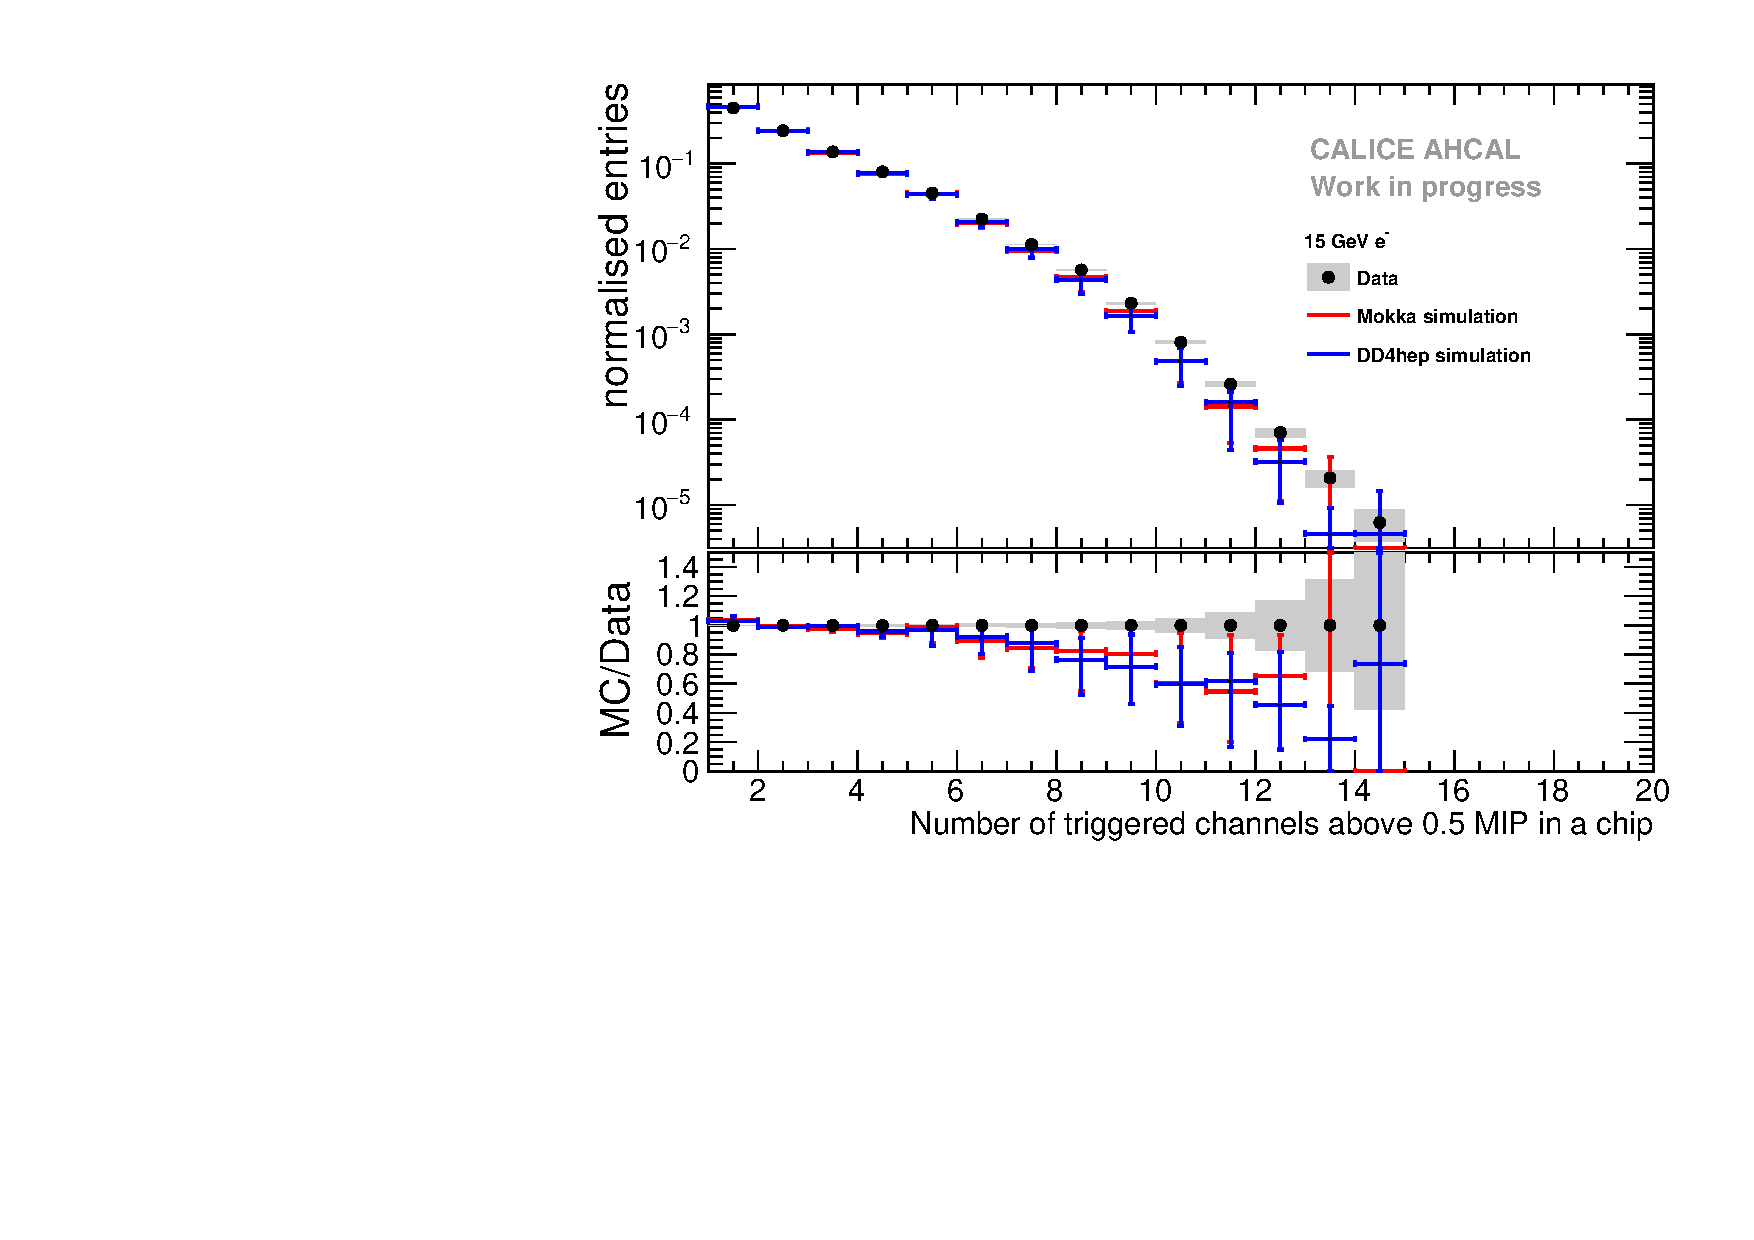
\includegraphics[width=1\textwidth]{../Thesis_Plots/Timing/Electrons/Plots/Comparison_SimData_Electrons_nHits_15GeV.pdf}
		\caption{15 GeV.}\label{fig:elec_sim_data_nHits_15GeV}
	\end{subfigure}
	\hfill
	\begin{subfigure}[t]{0.5\textwidth}
		\centering
		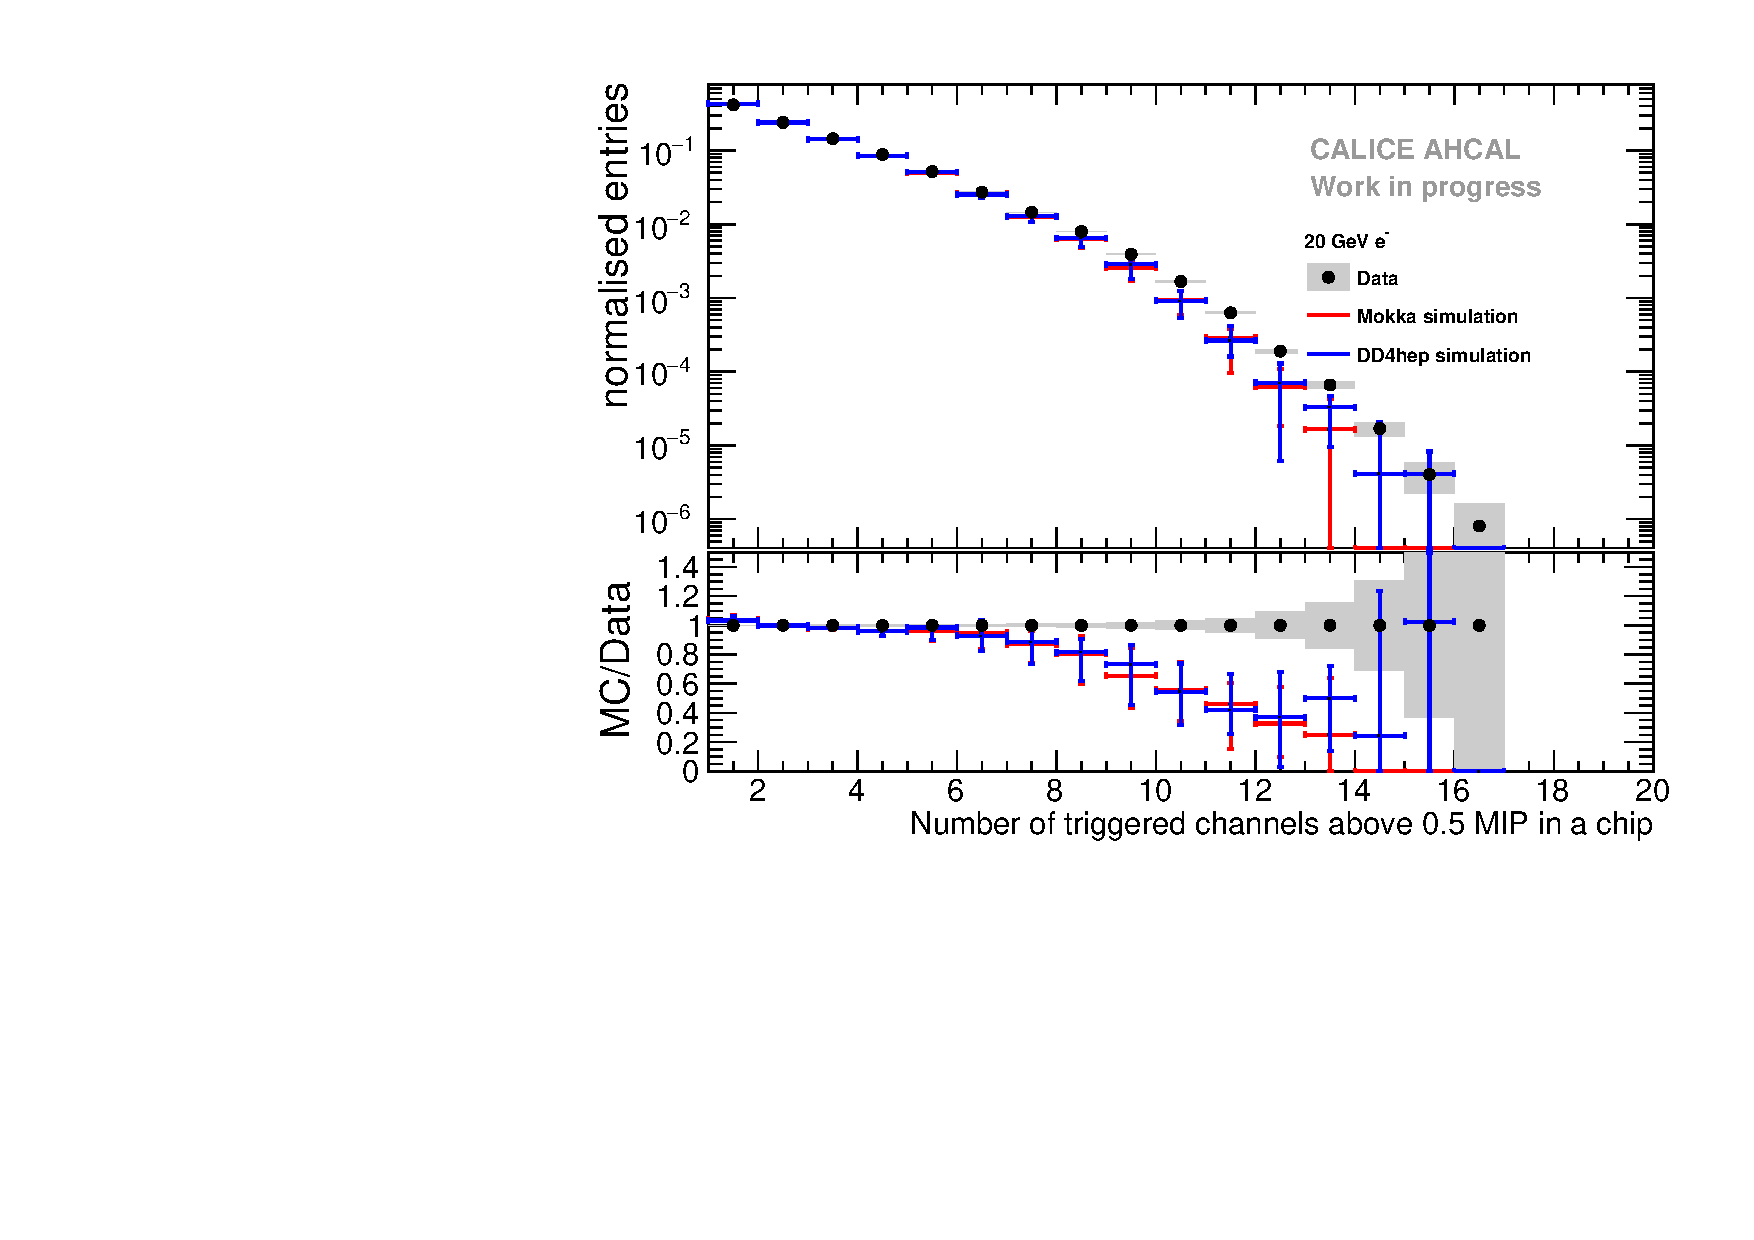
\includegraphics[width=1\textwidth]{../Thesis_Plots/Timing/Electrons/Plots/Comparison_SimData_Electrons_nHits_20GeV.pdf}
		\caption{20 GeV.}\label{fig:elec_sim_data_nHits_20GeV}
	\end{subfigure}
	\hfill
	\begin{subfigure}[t]{0.5\textwidth}
		\centering
		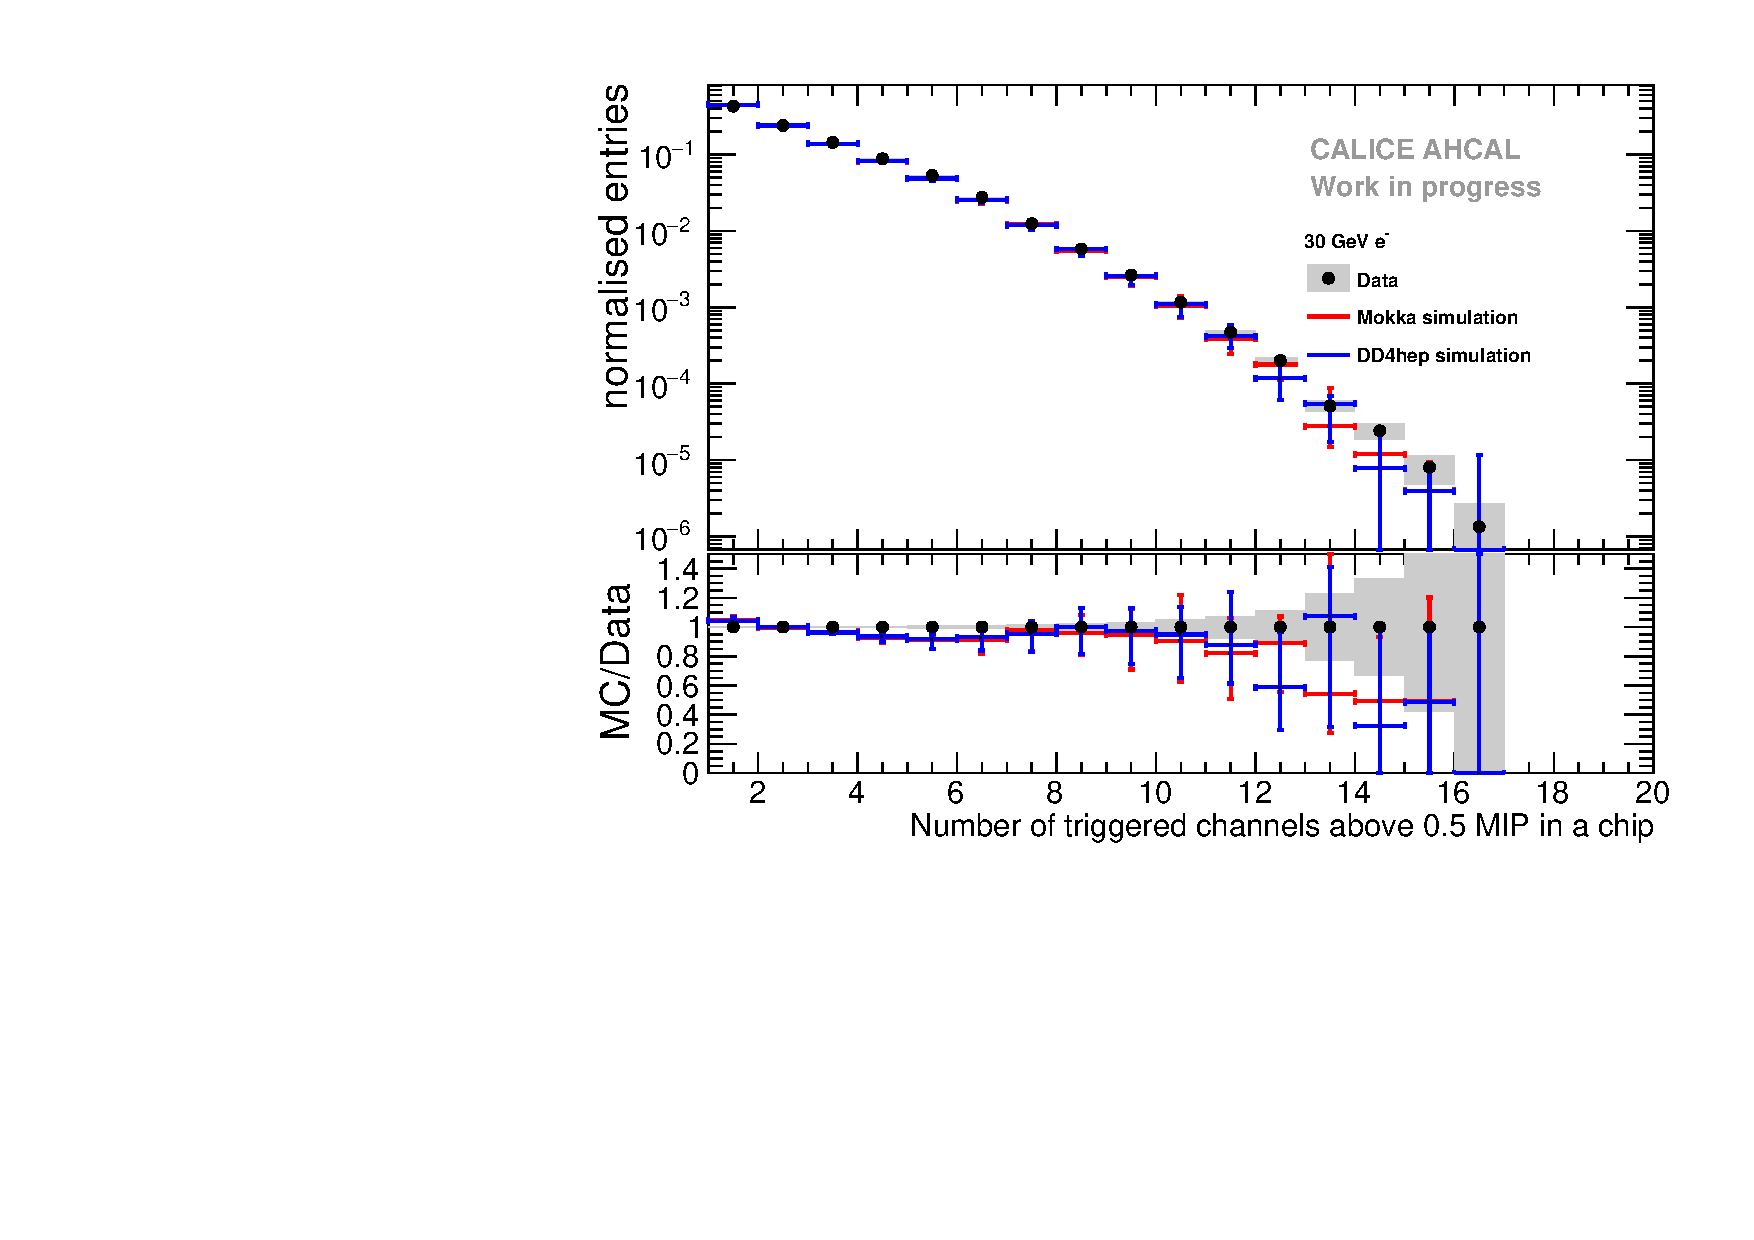
\includegraphics[width=1\textwidth]{../Thesis_Plots/Timing/Electrons/Plots/Comparison_SimData_Electrons_nHits_30GeV.pdf}
		\caption{30 GeV.}\label{fig:elec_sim_data_nHits_30GeV}
	\end{subfigure}
	\hfill
	\begin{subfigure}[t]{0.5\textwidth}
		\centering
		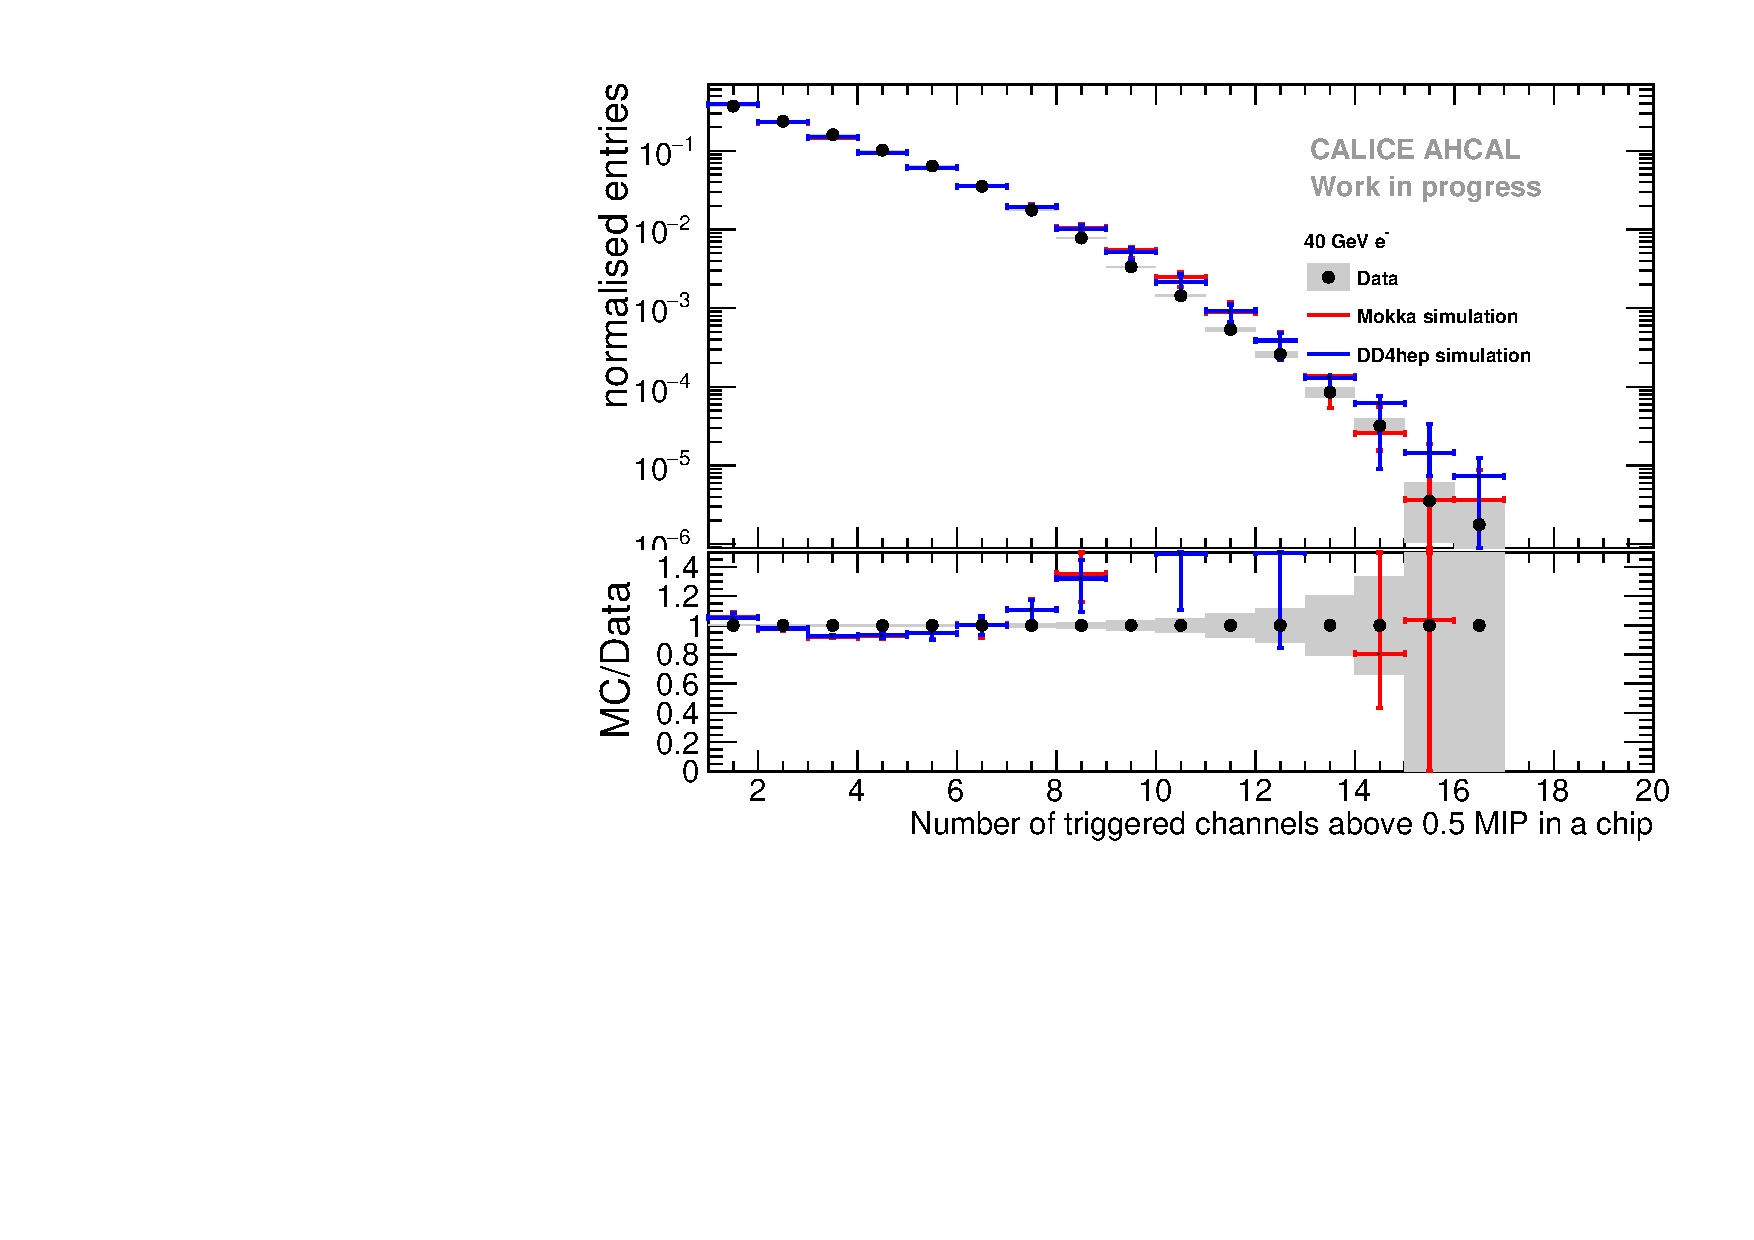
\includegraphics[width=1\textwidth]{../Thesis_Plots/Timing/Electrons/Plots/Comparison_SimData_Electrons_nHits_40GeV.pdf}
		\caption{40 GeV.}\label{fig:elec_sim_data_nHits_40GeV}
	\end{subfigure}
	\hfill
	\begin{subfigure}[t]{0.5\textwidth}
		\centering
		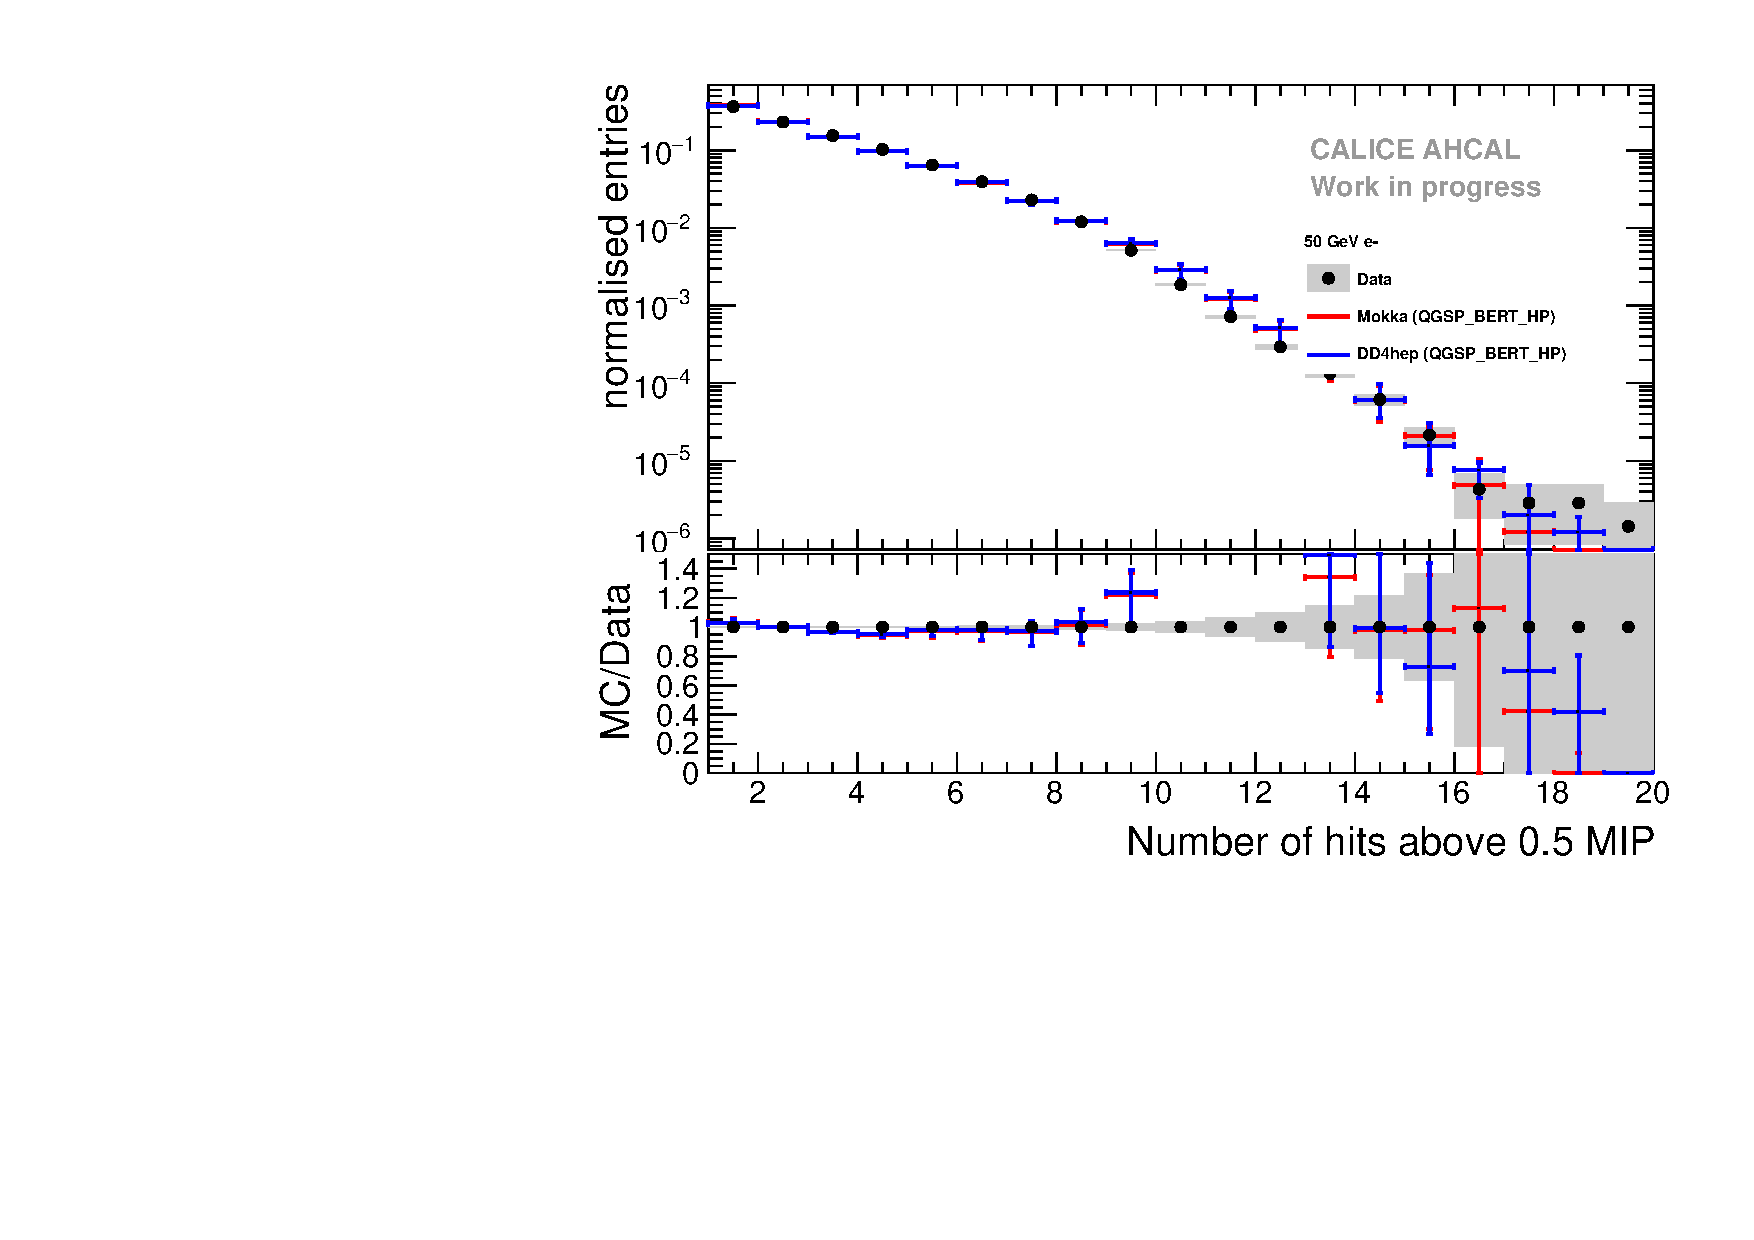
\includegraphics[width=1\textwidth]{../Thesis_Plots/Timing/Electrons/Plots/Comparison_SimData_Electrons_nHits_50GeV.pdf}
		\caption{50 GeV.}\label{fig:elec_sim_data_nHits_50GeV}
	\end{subfigure}
	\caption{Comparison between electron data and MC for all energies of the number of triggered channels per chip. The grey area represents the statistical error of the data. Error bars in simulation are obtained by varying the cross-talk parameter between 10\% and 18\%.}
	\label{fig:sim_data_elec_nHits}
\end{figure}
